\documentclass{article}
\PassOptionsToPackage{numbers,compress}{natbib}
\usepackage{neurips_2026}

\usepackage[utf8]{inputenc}
\usepackage[T1]{fontenc}
\usepackage{hyperref}
\hypersetup{pdfauthor={},pdftitle={},pdfsubject={},pdfkeywords={}} % 清理 PDF metadata，双盲审稿
\usepackage{url}
\usepackage{booktabs}
\usepackage{amsfonts}
\usepackage{amsmath}
\usepackage{nicefrac}
\usepackage[verbose=silent]{microtype}
\usepackage{xcolor}
\usepackage{graphicx}
\usepackage{subcaption}
\usepackage{multirow}
\usepackage{algorithm}
\usepackage{algorithmic}
\usepackage{xspace}
\providecommand{\bigtimes}{\mathop{\mathchoice{\textstyle\prod}{\prod}{\prod}{\prod}}\nolimits}  % fallback if stmaryrd unavailable
\usepackage{tikz}
\usetikzlibrary{arrows.meta,positioning,shapes.geometric,fit,backgrounds,patterns,calc}
\usepackage{pgfplots}
\pgfplotsset{compat=1.18}
\usepgfplotslibrary{fillbetween}

% 排版优化（合规：不改 margins/字体，只调间距）
\usepackage[font=small,labelfont=bf]{caption}      % caption 字体缩小，标签加粗
\setlength{\abovecaptionskip}{5pt}                  % caption 上方间距（默认 10pt）
\setlength{\belowcaptionskip}{2pt}                  % caption 下方间距（默认 0pt）
\setlength{\floatsep}{8pt plus 2pt minus 2pt}       % 连续浮动体之间（默认 12pt）
\setlength{\textfloatsep}{10pt plus 2pt minus 2pt}  % 浮动体与正文之间（默认 20pt）
\setlength{\intextsep}{6pt plus 2pt minus 2pt}      % [h] 浮动体与正文（默认 12pt）
\setlength{\abovedisplayskip}{6pt plus 2pt minus 2pt}   % 公式上方
\setlength{\belowdisplayskip}{6pt plus 2pt minus 2pt}   % 公式下方
\renewcommand{\figurename}{Fig.}                    % 缩写
\renewcommand{\tablename}{Tab.}

% 紧凑列表
\usepackage{enumitem}
\setlist[itemize]{itemsep=1pt, parsep=0pt, topsep=2pt}
\setlist[enumerate]{itemsep=1pt, parsep=0pt, topsep=2pt}

% 自定义命令
\newcommand{\method}{PCD}
\newcommand{\taskspec}{TaskSpec}
\newcommand{\eg}{e.g.,\xspace}
\newcommand{\ie}{i.e.,\xspace}
\newcommand{\etal}{\textit{et al.}\xspace}

% Internal review commands removed for double-blind submission

\title{Compile Once, Reason Exactly: Verified Solver Induction for LLM Probabilistic Reasoning}

% Camera-ready: 改 \usepackage[final]{neurips_2026} 并取消下方注释
% \author{
%   Bowen Jiang\quad
%   Xuan Wei\quad
%   Tao Yao\thanks{Corresponding author.} \\
%   Antai College of Economics and Management, Shanghai Jiao Tong University \\
%   \texttt{\{tree06, weix, taoyao\}@sjtu.edu.cn}
% }
\author{Anonymous Author(s)}

\begin{document}

\maketitle

% ============================================================
\begin{abstract}
% ============================================================
Large language models (LLMs) are increasingly asked to reason under uncertainty, but current systems treat each probabilistic benchmark as a separate prompting or tool-use problem.
We argue that the missing abstraction is a reusable \emph{probabilistic compiler}: an LLM should infer the mathematical structure of a task family once, emit a typed specification, and let a validated deterministic backend perform all subsequent inference.
We motivate this design with Parse--Compute--Decide (PCD), a gold-injection diagnostic across six models and several probabilistic tasks.
LLMs can often read the problem and act on a posterior, but their direct probabilistic computation is the weak link: Compute accuracy ranges from 22\% to 78\% on preference learning and drops to 3--11\% on depth-10 Bayesian networks, while structured natural-language parsing can itself become the bottleneck on harder inputs.
We implement the compiler abstraction with a declarative \taskspec{} interface, seven typed probabilistic operations, three reusable macros, and a deploy check for candidate solvers.
The same interface covers preference learning, bandits, Bayesian networks, Naive Bayes, and HMM forward filtering.
We report evidence in layers.
Given a valid specification, the deterministic backend matches reference solvers on 1,150 Flight/BLInD instances and 400 finite-query bnlearn checks, while larger bnlearn networks expose where per-instance code generation becomes unreliable.
In the realistic natural-language pipeline, GPT-4o-mini improves from 44\% / 32\% direct accuracy to \textbf{91.7\% / 98.0\%} on adversarial Naive Bayes and HMM inputs, two families with no built-in macro.
The central result is therefore not another high-accuracy prompt: it is a division of labor in which cheap LLMs emit reusable probabilistic specifications, and deterministic solvers carry the computation.
\end{abstract}

% ============================================================
\section{Introduction}
\label{sec:intro}
% ============================================================

Probabilistic reasoning is central to many applications where LLMs are now deployed, from medical diagnosis to portfolio management: given observed data, compute a posterior, then choose an action under uncertainty.
The underlying Bayesian computation is mathematically well understood but surprisingly hard for current language models.

Consider a concrete example: ask a frontier language model to perform variable elimination on a ten-node Bayesian network, and it will get the answer wrong 89\% of the time.
Yet ask it to \emph{identify the variables, parse the conditional probability tables, and state the query}, and it succeeds on 99\% of instances~\citep{nafar2025blind}.
The model understands the problem but cannot do the math.

The pattern is consistent across tasks.
On preference learning~\citep{qiu2026bayesian}, BN inference~\citep{nafar2025blind}, and multi-armed bandits~\citep{lim2025textbandit}, LLMs fall short of Bayesian oracles by 20--60 percentage points, even when they correctly recognize the problem structure.
Current fixes are task-specific: ProbLog for Bayesian networks~\citep{nafar2025blind,deraedt2007problog}, fine-tuning for preference tasks~\citep{qiu2026bayesian}. Each new task demands a new tool.
This is the abstraction gap we target.
Rather than teach the model to execute every probabilistic algorithm in-context, we ask it to produce a typed, reusable specification of \emph{what inference family this is}.
The backend then performs the inference exactly and repeatably.

To pinpoint where reasoning breaks down, we introduce \emph{Parse--Compute--Decide} (\method{}), a diagnostic that isolates each stage by injecting gold intermediate results.
\textbf{Parse} asks whether the model can extract problem structure;
\textbf{Compute$\mid$GoldParse} gives it perfect structure and tests the computation;
\textbf{Decide$\mid$GoldPosterior} gives it the correct posterior and tests whether it can act on it.

Across six models from OpenAI, Anthropic, and Google, Parse accuracy is 82--100\% on primary preference-learning tasks and Decide accuracy is 100\%, but Compute accuracy is only 22--78\%; on harder structured-input tasks (Naive-Bayes natural language), exact-match Parse drops sharply (Section~\ref{sec:held_out}).
The gap widens with problem complexity: GPT-5.4 computes the correct probability only 11\% of the time on depth-10 Bayesian networks, despite parsing the network perfectly.
Computation, not language understanding, is the bottleneck.

LLMs can identify \emph{what} to compute; the difficulty is \emph{how}. We therefore separate these two jobs (Figure~\ref{fig:overview}).
Given a new task, the LLM infers the mathematical structure of its task family once. A deterministic compiler then turns that description into an exact solver that requires no further LLM calls.
This demands more than instance-level parsing: the LLM must recognize the inference family, decide whether to reuse a built-in macro or represent the family through typed primitives, and emit a complete declarative specification. We validate this empirically, including on two held-out families represented without a built-in macro.

We implement this with a typed probabilistic DSL of seven core operations, a deterministic compiler, and a two-gate deploy check.
The same seven primitives express all five inference families we evaluate (preference, bandit, BN, Naive Bayes, HMM)---one library, not one tool per task.
Because the LLM fills a structured specification instead of writing arbitrary code, even GPT-4o-mini, the cheapest model we test, can produce reusable solvers whose compute stage matches hand-written references across 1,150 test instances (Flight 250, BLInD 900); the same variable-elimination backend also matches pgmpy references on 400 finite bnlearn queries.
This is a conditional backend result: it measures exactness after a valid \taskspec{} has been induced, while the end-to-end experiments separately measure natural-language specification extraction.
On natural-language inputs, the pipeline matches the gold-feature oracle at 74\% accuracy on preference learning and reaches 91.7\% / 98.0\% on adversarial held-out Naive Bayes / HMM inputs; see Sections~\ref{sec:e2e} and~\ref{sec:held_out}.

\textbf{Contributions.}
\begin{itemize}
    \item \textbf{A probabilistic compiler abstraction for LLM reasoning}: a declarative \taskspec{} interface, seven typed operations, three reusable macros, and a deterministic backend that together turn LLM structure recognition into reusable probabilistic solvers. The abstraction spans five tested inference families rather than one benchmark-specific tool.
    \item \textbf{A layered empirical case that separates specification from computation}: backend exactness is reported only conditional on a valid \taskspec{} (including 400/400 finite bnlearn checks), while natural-language E2E is measured separately on preference learning and on two held-out no-macro families (Naive Bayes and HMM: 91.7\% / 98.0\%).
    \item \textbf{A diagnostic for why LLM probabilistic reasoning fails}: gold-injection interventions (Parse, Compute, Decide) across six models, three vendors, and multiple task families isolate computation as the primary failure mode, while also showing where structured parsing itself becomes the limiting step.
\end{itemize}

\begin{figure*}[t]
\centering
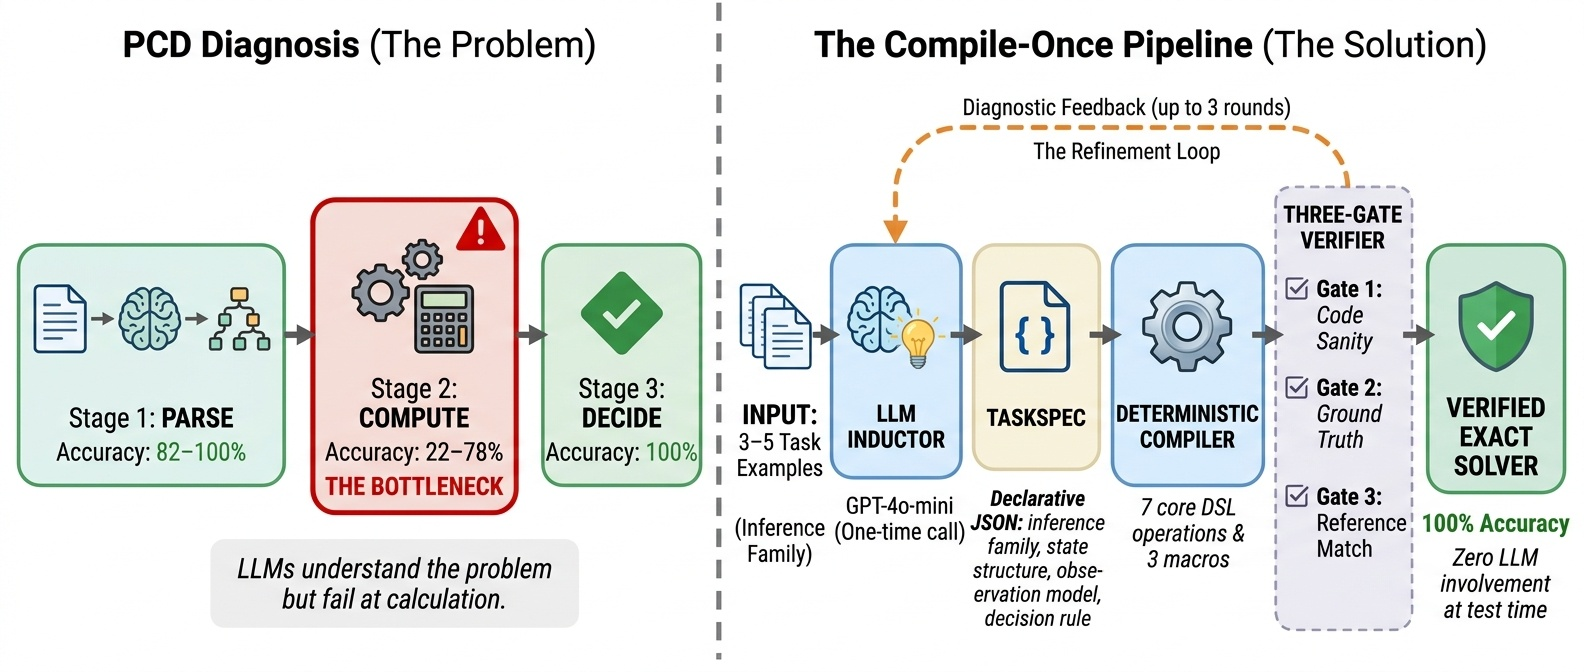
\includegraphics[width=\textwidth]{figures/figure1_overview.png}
\caption{Compile-once architecture with router-mediated reuse. Mixed natural-language inputs first pass through a scope/family router, which either rejects unsupported tasks or routes supported families to induction and reuse. When no solver is available, an LLM inductor emits a declarative \taskspec{}; a deterministic compiler lowers it to typed operations or core-op-backed routes, and a two-gate deploy check validates primary-family solvers when held-out labels are available. Validated solvers are stored in a reusable registry so later same-family instances can bypass LLM induction and execute deterministically.}
\label{fig:overview}
\end{figure*}

% ============================================================
\section{Problem Setup}
\label{sec:background}
% ============================================================

Our tasks share a common skeleton~\citep{griffiths2008bayesian,koller2009pgm}: observe data $\mathbf{x}$, compute a posterior $p(\theta \mid \mathbf{x}) \propto p(\mathbf{x} \mid \theta)\, p(\theta)$, and act via $a^* = \arg\max_a \mathbb{E}_{p(\theta \mid \mathbf{x})}[u(a, \theta)]$.
What varies is the \emph{inference family}: hypothesis enumeration for preference learning, conjugate update for bandits, or variable elimination for BN inference.
We evaluate on Flight/Hotel ($n{=}748$), TextBandit-style histories ($n{=}100$), BLInD ($n{=}900$), bnlearn (400 structured backend checks plus a 120-query PAL stress test), and an all-family mixed E2E benchmark ($n{=}650$).
Two additional families, Naive Bayes ($n{=}200$) and HMM forward filtering ($n{=}100$), are held out for generalization testing; see Appendix~\ref{app:families} for the full family table.

Prior work documents the failures: LLMs perform poorly on BN queries without tools~\citep{nafar2025blind}, symbolic solvers outperform them by wide margins~\citep{schrader2024quite}, even basic probability estimation is unreliable~\citep{paruchuri2024odds}, and chain-of-thought prompting~\citep{wei2022cot,wang2023selfconsistency} can further degrade performance on probabilistic tasks, as we confirm in \S\ref{sec:analysis}.
None of these studies separate parsing, computation, and decision-making as distinct failure modes. PCD fills this gap.

% ============================================================
\section{PCD: Diagnosing the Compute Bottleneck}
\label{sec:pcd}
% ============================================================

\subsection{Method: Gold-Injection Interventions}

We decompose probabilistic reasoning into three stages with well-defined interfaces.
The decomposition is general as a diagnostic template: any reasoning task with a parse--compute--decide structure could be probed by defining a gold oracle for each stage. We instantiate and validate it here for probabilistic inference, leaving mathematical proof, planning, and causal inference as possible future applications.
For a problem instance $x$ from family $F$, the gold computation pipeline is:
\begin{equation}
s^* = \mathcal{P}^*(x), \qquad y^* = \mathcal{C}^*(s^*), \qquad a^* = \mathcal{D}^*(y^*) = \arg\max_{a \in \mathcal{A}}\; \mathbb{E}_{p(\theta \mid \text{obs}(s^*))}[u(a, \theta)],
\label{eq:gold_pipeline}
\end{equation}
where $s^* = (\mathcal{V}, \mathcal{E}, \{\phi_i\}, Q, \mathbf{e})$ is the structured representation covering variables, edges, CPT factors, query, and evidence; $y^*$ is the exact posterior or expected utilities; and $a^*$ is the optimal action.
An LLM $\psi$ implements approximate versions $P_\psi$, $C_\psi$, $D_\psi$ of each stage, yielding $\hat{a} = D_\psi(C_\psi(P_\psi(x)))$.
PCD isolates each stage via gold-injection interventions:
\begin{align}
\text{ParseAcc}_\psi &= \frac{1}{|\mathcal{D}|}\sum_{x \in \mathcal{D}} \prod_{f \in \mathcal{F}} \mathbf{1}\!\left\{P_\psi^{(f)}(x) = s^{*(f)}\right\}, \label{eq:parse}\\[4pt]
\text{CompAcc}_\psi &= \frac{1}{|\mathcal{D}|}\sum_{x \in \mathcal{D}} \mathbf{1}\!\left\{\left\|C_\psi\!\left(\mathcal{P}^*(x)\right) - \mathcal{C}^*\!\left(\mathcal{P}^*(x)\right)\right\|_\infty < \epsilon\right\}, \label{eq:compute}\\[4pt]
\text{DecAcc}_\psi &= \frac{1}{|\mathcal{D}|}\sum_{x \in \mathcal{D}} \mathbf{1}\!\left\{D_\psi\!\left(\mathcal{C}^*(s^*)\right) = a^*\right\}, \label{eq:decide}
\end{align}
where $\mathcal{F}$ indexes the structural fields (variables, edges, CPTs, query, evidence) and Parse is scored correct only when \emph{all} fields match.
A signature of $\text{ParseAcc} \approx 1,\; \text{DecAcc} \approx 1,\; \text{CompAcc} \ll 1$ indicates a compute bottleneck.
We observe this pattern across every model and task.

\subsection{Results: A Consistent Compute Bottleneck}

On preference learning, Compute ranges from 28\% for GPT-4o-mini to 78\% for Opus, while Decide = 100\% for every model.
On BN inference, the same pattern holds and amplifies with depth: Compute drops from $\sim$82\% at depth 2 to single digits by depth 10, while Parse stays $\geq$96\% and Decide at 100\%.

\begin{figure*}[t]
\centering
\begin{minipage}[t]{0.38\textwidth}
\vspace{0pt}
\centering
\small
\captionof{table}{PCD on preference learning (Flight, $n{=}200$). Parse $\geq$82\% and Decide = 100\% for all models, but Compute peaks at 78\% (Opus) and is only 28\% for GPT-4o-mini. 95\% CIs in brackets.}
\label{tab:pcd_preference}
\vspace{4pt}
\begin{tabular}{@{}lcc@{}}
\toprule
Model & Parse & Compute$\mid$Gold \\
\midrule
GPT-4o-mini & 82\% & 28\% {\scriptsize [21,34]} \\
GPT-4o & 100\% & 30\% {\scriptsize [23,36]} \\
GPT-5.4 & 100\% & 40\% {\scriptsize [33,47]} \\
Sonnet 4 & 100\% & 64\% {\scriptsize [57,71]} \\
Gemini 3.1 & 100\% & 69\% {\scriptsize [62,75]} \\
Opus 4.6 & 100\% & 78\% {\scriptsize [71,83]} \\
\midrule
Our DSL & --- & 100\% \\
\bottomrule
\end{tabular}
\end{minipage}\hfill
\begin{minipage}[t]{0.59\textwidth}
\vspace{0pt}
\centering
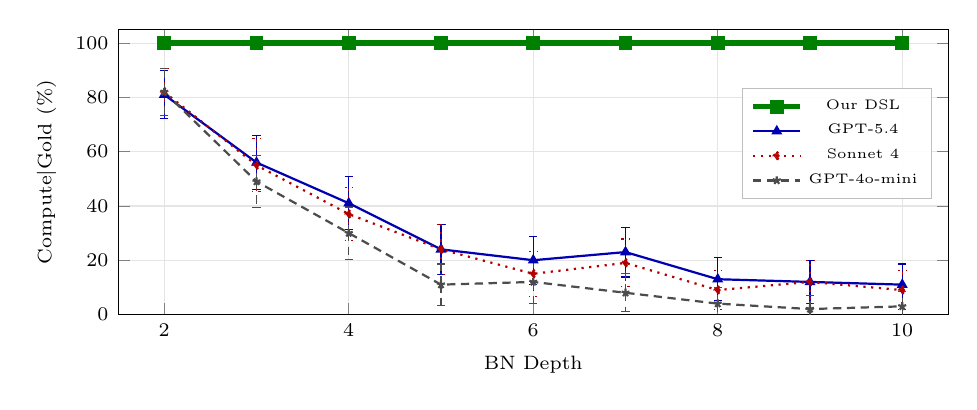
\begin{tikzpicture}
\begin{axis}[
    width=\textwidth,
    height=5.2cm,
    xlabel={BN Depth},
    ylabel={Compute$\mid$Gold (\%)},
    xmin=1.5, xmax=10.5,
    ymin=0, ymax=105,
    xtick={2,4,6,8,10},
    ytick={0,20,40,60,80,100},
    legend style={at={(0.98,0.60)}, anchor=east, font=\tiny, draw=gray!50, fill=white, fill opacity=0.9, text opacity=1, row sep=0pt},
    grid=major,
    grid style={gray!20},
    tick label style={font=\scriptsize},
    label style={font=\scriptsize},
    every axis plot/.append style={thick, mark size=1.5pt},
]
\addplot[color=green!50!black, line width=2pt, solid, mark=square*, mark options={fill=green!50!black}]
    coordinates {(2,100)(3,100)(4,100)(5,100)(6,100)(7,100)(8,100)(9,100)(10,100)};
\addlegendentry{Our DSL}
% GPT-5.4 with Wilson 95% CI error bars (n=100 per depth)
\addplot[color=blue!70!black, mark=triangle*, mark options={fill=blue!70!black},
    error bars/.cd, y dir=both, y explicit]
    coordinates {
        (2,81) +- (0,8.8) (3,56) +- (0,9.8) (4,41) +- (0,9.8)
        (5,24) +- (0,9.2) (6,20) +- (0,8.9) (7,23) +- (0,9.2)
        (8,13) +- (0,8.0) (9,12) +- (0,7.8) (10,11) +- (0,7.6)
    };
\addlegendentry{GPT-5.4}
% Sonnet 4 with Wilson 95% CI
\addplot[color=red!70!black, dotted, mark=diamond*, mark options={fill=red!70!black},
    error bars/.cd, y dir=both, y explicit]
    coordinates {
        (2,82) +- (0,8.7) (3,55) +- (0,9.8) (4,37) +- (0,9.8)
        (5,24) +- (0,9.2) (6,15) +- (0,8.3) (7,19) +- (0,8.8)
        (8,9) +- (0,7.2) (9,12) +- (0,7.8) (10,9) +- (0,7.2)
    };
\addlegendentry{Sonnet 4}
% GPT-4o-mini with Wilson 95% CI
\addplot[color=gray!60!black, densely dashed, mark=star, mark options={fill=gray!60!black},
    error bars/.cd, y dir=both, y explicit]
    coordinates {
        (2,82) +- (0,8.7) (3,49) +- (0,9.7) (4,30) +- (0,9.6)
        (5,11) +- (0,7.6) (6,12) +- (0,7.8) (7,8) +- (0,7.0)
        (8,4) +- (0,5.8) (9,2) +- (0,5.0) (10,3) +- (0,5.5)
    };
\addlegendentry{GPT-4o-mini}
\end{axis}
\end{tikzpicture}
\captionof{figure}{Compute$\mid$GoldParse accuracy vs.\ BN depth (BLInD, $n{=}900$, 100 per depth). Error bars show 95\% Wilson CIs. All three LLMs degrade from $\sim$82\% at depth~2 to single digits by depth~10; our DSL solver maintains 100\% at every depth.}
\label{fig:depth}
\end{minipage}
\end{figure*}

The pattern is consistent across every model and task family, including two held-out families (Naive Bayes and HMM forward filtering) evaluated in \S\ref{sec:held_out}.
Scaling helps, but not enough: upgrading from GPT-4o-mini to GPT-5.4 (a $67\times$ price increase) improves Compute by only 9 percentage points on BN inference.
At depth 10, GPT-5.4 still produces the wrong answer 89\% of the time.
These results motivate a system that uses the LLM's strong parsing ability while bypassing its weak computation entirely.

% ============================================================
\section{Method: Typed DSL and Verified Solver Induction}
\label{sec:method}
% ============================================================

PCD reveals that computation, not parsing, limits LLM probabilistic reasoning.
We now ask whether LLMs can use their parsing strength differently: given a new task, can they infer the mathematical structure of an entire task \emph{family}?
That is a stronger capability than instance-level parsing, and we test it empirically.

Given a new task family, an LLM inductor receives a small labeled example set and emits a declarative \taskspec{} rather than executable code.
The deterministic compiler lowers that specification into a solver; if the solver fails a deploy check, diagnostic feedback can trigger a bounded number of refinement rounds (Algorithm~\ref{alg:pipeline}).
The deploy check has two gates when held-out validation labels are available: the solver must execute, and its outputs must match those validation labels within the appropriate tolerance.
We evaluate the resulting solver on unseen instances from the same family, using exact match for discrete decisions and absolute error for probabilities.
At test time, the compiled solver runs without any LLM involvement, producing deterministic outputs.

\subsection{Probabilistic DSL}

The DSL has two layers.

\paragraph{Core Operations (7 typed ops).}
The minimal building blocks for discrete probabilistic computation:
\texttt{condition}, \texttt{multiply}, \texttt{marginalize}, \texttt{normalize}, \texttt{enumerate\_hypotheses}, \texttt{expectation}, \texttt{argmax}.
Each operation has a precise type signature (\eg{} \texttt{normalize: Factor $\to$ Distribution}; full signatures in Appendix~\ref{app:dsl}).

\paragraph{Family Macros (syntactic sugar).}
Three macros compose core operations for common inference patterns: \texttt{softmax\_pref} (hypothesis enumeration), \texttt{beta\_bernoulli} (conjugate update), \texttt{ve\_query} (variable elimination).
For example, VE computes the query posterior by iterated factor elimination:
\begin{equation}
P(Q{=}q \mid \mathbf{E}{=}\mathbf{e}) = \frac{1}{Z} \sum_{\mathbf{H}} \prod_{i=1}^{n} \phi_i(\mathbf{x}_i)\Big|_{\mathbf{E}=\mathbf{e},\, Q=q}, \quad Z = \sum_{q'}\sum_{\mathbf{H}} \prod_{i=1}^{n} \phi_i(\mathbf{x}_i)\Big|_{\mathbf{E}=\mathbf{e},\, Q=q'},
\label{eq:ve}
\end{equation}
where $\phi_i$ are the CPT factors and $\mathbf{H}$ are the hidden variables.
For preference learning, the posterior over weight vectors $\theta \in \Theta$ after $T$ sequential choices is:
\begin{equation}
p(\theta \mid \mathbf{c}_{1:T}) = \frac{p(\theta)\,\prod_{t=1}^{T} P(c_t \mid \theta, \mathbf{X}_t)}{\sum_{\theta' \in \Theta} p(\theta')\,\prod_{t=1}^{T} P(c_t \mid \theta', \mathbf{X}_t)}, \quad P(c_t \mid \theta, \mathbf{X}_t) = \frac{\exp(\theta^\top \mathbf{x}_{c_t})}{\sum_{j=1}^{J} \exp(\theta^\top \mathbf{x}_{j,t})},
\label{eq:pref}
\end{equation}
and the optimal recommendation maximizes expected utility: $a^* = \arg\max_{j} \sum_{\theta} p(\theta \mid \mathbf{c}_{1:T})\, \theta^\top \mathbf{x}_j$.
Macros are not the only route through the interface: for two held-out families with no corresponding macro, extended \taskspec{} fields and core-op-backed solvers are exact given a valid specification, and the full adversarial-NL pipeline reaches 91.7\% / 98.0\% with the residual gap attributable to LLM specification-extraction errors on hedged numerals.

\subsection{TaskSpec: Declarative Intermediate Representation}

A \taskspec{} is a JSON document that declares a task's mathematical structure: inference family, state space, observation model, and decision rule.
The LLM inductor outputs a \taskspec{}; it never writes executable code.
For example, given 3 flight-recommendation episodes, GPT-4o-mini emits a \taskspec{} specifying \texttt{hypothesis\_enumeration} over a 4-feature preference space with softmax choice likelihood.
From this, the compiler produces a solver that enumerates all $5^4 = 625$ weight vectors, updates a posterior via softmax likelihoods after each user choice, and recommends the option maximizing expected utility (see Appendix~\ref{app:taskspec} for the full schema).

\paragraph{Compile-once regime.}
The inductor is called once per \emph{inference family}, not per problem instance.
The resulting solver handles new instances from the same family, including varying topologies, feature counts, and observation lengths.
If the two-gate verifier rejects the compiled solver, diagnostic feedback triggers up to 3 refinement rounds (Algorithm~\ref{alg:pipeline}).
Once validated, the solver is deployed without further LLM calls.

\paragraph{Router and reusable registry.}
For the mixed E2E setting, a lightweight scope/family router first maps an input to one of the supported families or to an unsupported-reject branch.
This router is evaluated only in the bounded setting described in \S\ref{sec:all_family_mixed}; it is not an open-world solvability detector.
After a family-level solver has been validated, the implementation stores it in a reusable registry keyed by family and schema.
Later same-family instances can then route directly to the stored solver, bypassing LLM induction while still using LLM parsing when natural-language fields must be extracted.
Automatically growing this registry into a self-evolving macro library is a future extension, not a claim evaluated in this paper.

\subsection{Deterministic Compiler}

The compiler translates a \taskspec{} into an executable solver composed exclusively of DSL primitives.
Because both the schema and the operations are explicitly defined, the compiler is deterministic: the same specification always yields the same solver.
Compiled solvers match independent gold-reference implementations on BN queries, with maximum absolute error below $10^{-12}$ (floating-point precision) across all 1,150 test instances spanning Flight~250 and BLInD~900, where ground-truth posteriors are taken directly from the BLInD dataset; see Appendix~\ref{app:equivalence}.
Because the compiled solver is deterministic and reference-matched on these finite checks, 100\% backend accuracy should be read as a conditional exact-computation result, not as an open-ended natural-language accuracy claim.

\subsection{Verifier-Guided Inductor}

Given a new task, the inductor performs three steps in a single LLM call:
\begin{enumerate}[leftmargin=*]
    \item \textbf{Family recognition.} The inductor identifies the inference family from the examples---hypothesis enumeration, conjugate update, variable elimination, or none of the above.
    \item \textbf{Route decision.} If the recognized family matches a built-in macro, the inductor selects it and fills the corresponding \taskspec{} fields. If no macro matches, the family is represented through explicit \taskspec{} fields and a core-op-backed route. For HMM forward filtering, this route uses an iterated \texttt{multiply}$\to$\texttt{marginalize}$\to$\texttt{normalize} loop over a time axis, a sequential pattern absent from all three built-in macros (\S\ref{sec:held_out}).
    \item \textbf{Specification emission.} The inductor outputs a complete \taskspec{} JSON.
\end{enumerate}
Table~\ref{tab:routes} shows the route for each tested family. Three families reuse macros; two use core-op-backed routes, which tests whether the \taskspec{} interface can represent families beyond the initial macro library rather than merely selecting a benchmark-specific template.

\begin{table}[t]
\centering
\small
\caption{Inductor routes. Families with a matching macro reuse it; held-out families are represented through explicit \taskspec{} fields and core-op-backed solver routes rather than a built-in macro.}
\label{tab:routes}
\begin{tabular}{@{}llll@{}}
\toprule
Family & Macro & Route & Core-op-backed path \\
\midrule
Flight/Hotel & \texttt{softmax\_pref} & Macro reuse & --- \\
TextBandit & \texttt{beta\_bernoulli} & Macro reuse & --- \\
BLInD/bnlearn & \texttt{ve\_query} & Macro reuse & --- \\
\midrule
Naive Bayes & \emph{none} & Core-ops & enum $\to$ mult $\to$ norm $\to$ exp $\to$ argmax \\
HMM Forward & \emph{none} & Core-ops & iter(mult $\to$ marg $\to$ norm) over $t$ \\
\bottomrule
\end{tabular}
\end{table}

A two-gate verifier checks compiled solvers for primary deploy families when held-out validation labels are available:
\begin{enumerate}
    \item \textbf{Gate~1, Code Sanity}: The compiled solver executes without errors.
    \item \textbf{Gate~2, Ground Truth}: Solver outputs match known correct answers on held-out validation samples, disjoint from induction examples and the final test set.
\end{enumerate}
For NB/HMM held-out experiments, we report the natural-language E2E row and separate structured-spec backend sanity checks rather than claiming that the deploy verifier independently certifies those families.
If either deploy gate fails, diagnostic feedback guides the inductor to refine the \taskspec{}, up to 3 rounds.
Algorithm~\ref{alg:pipeline} summarizes the full compile-once pipeline.

\begin{algorithm}[t]
\caption{Compile-Once Solver Induction}
\label{alg:pipeline}
\begin{algorithmic}[1]
\REQUIRE Induction examples $\mathcal{D}_{\text{train}}$, validation examples $\mathcal{D}_{\text{val}}$ (disjoint)
\ENSURE Empirically validated solver $S$ or failure
\STATE $\textit{spec} \leftarrow \text{LLM}_{\text{induce}}(\mathcal{D}_{\text{train}})$ \COMMENT{GPT-4o-mini infers TaskSpec}
\FOR{$r = 1$ \TO $R_{\max}$}
    \STATE $S \leftarrow \textsc{Compile}(\textit{spec})$ \COMMENT{deterministic: TaskSpec $\to$ solver}
    \STATE $g_1 \leftarrow$ \textsc{Gate1\_Sanity}($S$) \COMMENT{compiled solver executes?}
    \IF{$\neg g_1$}
        \STATE $\textit{spec} \leftarrow \text{LLM}_{\text{refine}}(\textit{spec}, \text{diagnostics})$
        \STATE \textbf{continue}
    \ENDIF
    \STATE $g_2 \leftarrow$ \textsc{Gate2\_GroundTruth}($S, \mathcal{D}_{\text{val}}$) \COMMENT{outputs match gold on held-out?}
    \IF{$g_1 \wedge g_2$}
        \RETURN $S$ \COMMENT{validated solver deployed}
    \ENDIF
    \STATE $\textit{spec} \leftarrow \text{LLM}_{\text{refine}}(\textit{spec}, \text{diagnostics})$
\ENDFOR
\RETURN \textsc{Failure}
\end{algorithmic}
\end{algorithm}

\paragraph{Leave-One-Out (LOO) Generalization.}
We test the inductor on 6 held-out datasets spanning 3 inference families: Hotel, Flight-2F/3F/5F/6F, and BLInD depth-out-of-distribution.
All 6 pass the engineering sanity checks on the first attempt without self-refinement.
We treat this as a small implementation check, not as a main generalization result.

\paragraph{Inductor Reliability.}
To measure variance, we run the inductor 20 times per family on Flight and BN at temperature 0.7.
All 40 trials pass verification on the first attempt.
A single example at $k{=}1$ suffices for both families; we default to $k{=}3$--5 for robustness, but the system works with minimal supervision.
This reliability reflects the constrained output space: filling a declarative JSON specification is far easier than generating arbitrary probabilistic code.

% ============================================================
\section{Experiments}
\label{sec:experiments}
% ============================================================

We organize the evidence around three questions:
(1) do LLMs fail at probabilistic computation rather than merely at formatting or final choice?
(2) does a typed \taskspec{} interface provide a reusable backend across inference families?
(3) does the full natural-language pipeline remain useful when specification extraction is imperfect?
Table~\ref{tab:evidence_map} maps each claim to the evidence layer that supports it.

\begin{table}[t]
\centering
\small
\caption{Claim-to-evidence map. We separate backend exactness from natural-language E2E so that 100\% deterministic checks are not mistaken for open-ended LLM accuracy claims.}
\label{tab:evidence_map}
\begin{tabular}{@{}p{0.27\linewidth}p{0.34\linewidth}p{0.29\linewidth}@{}}
\toprule
Claim & Evidence & Scope \\
\midrule
LLMs have a compute bottleneck & PCD on preference learning and BLInD: Compute 22--78\%; depth-10 BN Compute 3--11\% & Diagnostic, not our system \\
Typed specs enable exact backend computation & Compiled solvers match references on Flight/BLInD ($n{=}1{,}150$); VE backend matches bnlearn finite-query references ($n{=}400$) & Conditional on a valid \taskspec{} or structured BN spec \\
The interface extends beyond built-in macros & Adversarial NL E2E on NB/HMM: 91.7\% / 98.0\% vs direct 44\% / 32\% & Two held-out synthetic families \\
The pipeline works on raw NL tasks & Flight 74.3\%, Hotel 77.4\%, TextBandit-style 96.0\% & Single-family full NL pipeline \\
Routing integrates with solving & Conservative all-family E2E aggregate: 90.4\% overall, 89.7\% supported solve & Six supported families plus unsupported rejection; router sanity checked separately \\
\bottomrule
\end{tabular}
\end{table}

We then report the detailed results in the same order.
Backend accuracy rows test whether the compiled solver is exact once a valid \taskspec{} exists; these rows can legitimately reach 100\% because the computation is deterministic.
End-to-end rows test the realistic LLM-facing pipeline, where errors can enter through family recognition or specification extraction.
This distinction is essential for interpreting the tables below: 100\% backend accuracy is a correctness check, while adversarial natural-language evaluations measure generalization of the induction interface.

\subsection{Baselines}

We compare against three baselines:

\begin{itemize}
    \item \textbf{Direct Answer}: LLM answers each problem instance directly (per-instance, no code).
    \item \textbf{Program-Aided Language Models (PAL)}~\citep{gao2023pal}: LLM generates a Python program per instance and executes it.
    \item \textbf{Compile-time Code Generation}: LLM sees 3--5 examples and writes a reusable Python solver, with up to 5 rounds of self-repair on training examples.
\end{itemize}

\subsection{Baselines on Synthetic Networks (BLInD)}

On BLInD's synthetic networks (2--10 binary nodes), PAL accuracy varies sharply with the underlying model: GPT-4o-mini collapses from 93\% at depth~2 to 2\% at depth~10 (Appendix~\ref{app:pal_depth}), while GPT-5.4 maintains 98.1\% overall (96\% at depth~10).
Among compile-time baselines, GPT-5.4 writes a working VE solver after one repair round, but GPT-4o-mini fails after five rounds, scoring 0\% on all 900 problems.
Our DSL sidesteps this entirely: GPT-4o-mini reaches 100\% through TaskSpec induction without writing any probabilistic code.

\subsection{Scaling to Real-World Networks}

BLInD's small binary networks are an ideal case for PAL: the generated code is short and the state space is tractable.
Real-world networks are larger, multi-valued, and harder to handle.
To test whether PAL holds up at scale, we evaluate on four standard bnlearn networks~\citep{scutari2010bnlearn}: Asia (8 nodes), Child (20 nodes, multi-valued), Insurance (27 nodes, 52 edges), and Alarm (37 nodes, 46 edges), all widely used PGM benchmarks with categorical variables taking up to 5 values.

On Asia, PAL with GPT-5.4 still reaches 90\%, but \textbf{on networks with $\geq$20 nodes it drops to 0\% on Child, 3\% on Insurance, and 0\% on Alarm}; GPT-4o-mini is low overall (17.5\%) and also reaches 0\% on Alarm (Figure~\ref{fig:scaling_cost}).
Only 27--29\% of generated programs execute successfully overall: the variable-elimination code often crashes on multi-valued CPTs, deep elimination chains, and complex factor products.
In contrast, the deterministic DSL backend matches pgmpy variable-elimination references on \textbf{400/400} finite bnlearn queries (100 per network; Wilson 95\% CI [99.0, 100.0]).
We therefore use bnlearn as a structured external backend check and a stress test for per-instance code generation, not as a natural-language E2E result.
The gap between per-instance generation and deterministic backends widens sharply as networks become larger and multi-valued.

\begin{figure*}[t]
\centering
% 两个子图，用 tabular 强制对齐
\begin{tabular}{@{}p{0.51\textwidth}@{\hspace{0.02\textwidth}}p{0.47\textwidth}@{}}
% ---- 子图 (a) ----
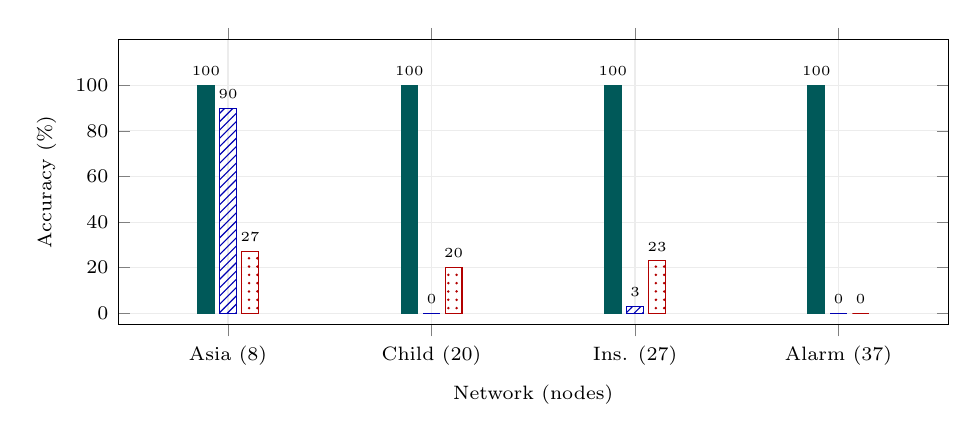
\begin{tikzpicture}
\begin{axis}[
    width=\linewidth,
    height=5.2cm,
    ybar,
    bar width=6pt,
    xlabel={Network (nodes)},
    ylabel={Accuracy (\%)},
    ymin=-5, ymax=120,
    ytick={0,20,40,60,80,100},
    symbolic x coords={Asia (8), Child (20), Ins. (27), Alarm (37)},
    xtick=data,
    x tick label style={font=\scriptsize},
    tick label style={font=\scriptsize},
    label style={font=\scriptsize},
    legend to name=legA,
    legend style={font=\tiny, draw=gray!50, legend columns=1, column sep=3pt},
    legend image code/.code={\draw[#1, draw=none] (0cm,-0.1cm) rectangle (0.25cm,0.15cm);},
    grid=major,
    grid style={gray!15},
    nodes near coords,
    every node near coord/.append style={font=\tiny, anchor=south},
    enlarge x limits=0.18,
]
\addplot[fill=teal!70!black, draw=teal!70!black] coordinates {(Asia (8),100) (Child (20),100) (Ins. (27),100) (Alarm (37),100)};
\addlegendentry{DSL backend}
\addplot[pattern=north east lines, pattern color=blue!70!black, draw=blue!70!black] coordinates {(Asia (8),90) (Child (20),0) (Ins. (27),3) (Alarm (37),0)};
\addlegendentry{PAL (5.4)}
\addplot[pattern=dots, pattern color=red!70!black, draw=red!70!black] coordinates {(Asia (8),27) (Child (20),20) (Ins. (27),23) (Alarm (37),0)};
\addlegendentry{PAL (GPT-4o-mini)}
\end{axis}
\end{tikzpicture}
&
% ---- 子图 (b) ----
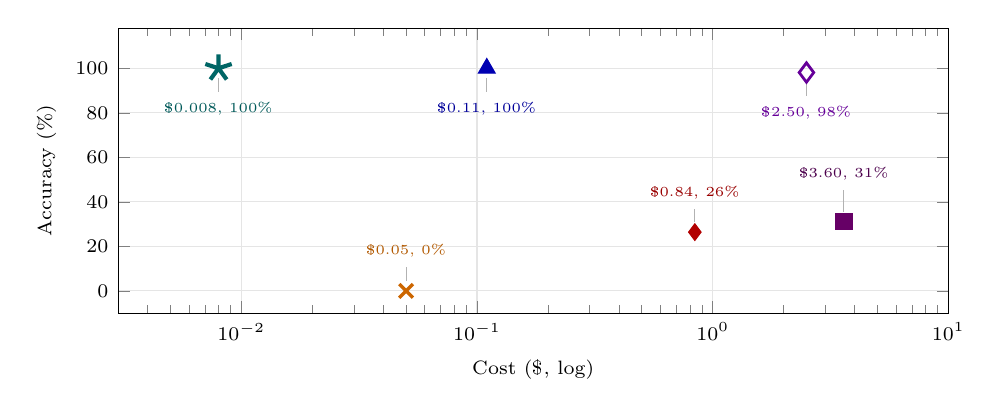
\begin{tikzpicture}
\begin{axis}[
    width=\linewidth,
    height=5.2cm,
    xlabel={Cost (\$, log)},
    ylabel={Accuracy (\%)},
    xmode=log,
    xmin=0.003, xmax=10,
    ymin=-10, ymax=118,
    ytick={0,20,40,60,80,100},
    grid=major,
    grid style={gray!20},
    tick label style={font=\scriptsize},
    label style={font=\scriptsize},
    legend to name=legB,
    legend style={font=\tiny, draw=gray!50, legend columns=3, column sep=3pt},
]
% 统一标签格式: 方法 (模型)
\addplot[only marks, mark=star, mark size=5pt, color=teal!80!black, line width=1.5pt]
    coordinates {(0.008, 100)};
\addlegendentry{Our DSL (GPT-4o-mini)}
\addplot[only marks, mark=triangle*, mark size=3.5pt, color=blue!70!black]
    coordinates {(0.11, 100)};
\addlegendentry{Compile (GPT-5.4)}
\addplot[only marks, mark=x, mark size=3.5pt, color=orange!80!black, line width=1.2pt]
    coordinates {(0.05, 0)};
\addlegendentry{Compile (GPT-4o-mini)}
\addplot[only marks, mark=diamond, mark size=3.5pt, color=red!40!blue, line width=1pt]
    coordinates {(2.50, 98.1)};
\addlegendentry{PAL (GPT-5.4)}
\addplot[only marks, mark=diamond*, mark size=3pt, color=red!70!black]
    coordinates {(0.84, 26.4)};
\addlegendentry{PAL (GPT-4o-mini)}
\addplot[only marks, mark=square*, mark size=3pt, color=violet!80!black]
    coordinates {(3.60, 31.2)};
\addlegendentry{Direct (GPT-5.4)}
% pin 标注：高分正下，低分正上
\node[pin={[pin distance=5pt, pin edge={gray!60, thin}, font=\tiny, text=teal!70!black]-90:{\$0.008, 100\%}}] at (axis cs:0.008,100) {};
\node[pin={[pin distance=5pt, pin edge={gray!60, thin}, font=\tiny, text=blue!60!black]-90:{\$0.11, 100\%}}] at (axis cs:0.11,100) {};
\node[pin={[pin distance=5pt, pin edge={gray!60, thin}, font=\tiny, text=red!40!blue]-90:{\$2.50, 98\%}}] at (axis cs:2.50,98.1) {};
\node[pin={[pin distance=5pt, pin edge={gray!60, thin}, font=\tiny, text=orange!70!black]90:{\$0.05, 0\%}}] at (axis cs:0.05,0) {};
\node[pin={[pin distance=5pt, pin edge={gray!60, thin}, font=\tiny, text=red!60!black]90:{\$0.84, 26\%}}] at (axis cs:0.84,26.4) {};
\node[pin={[pin distance=8pt, pin edge={gray!60, thin}, font=\tiny, text=violet!60!black]90:{\$3.60, 31\%}}] at (axis cs:3.60,31.2) {};
\end{axis}
\end{tikzpicture}
\\
% ---- 外部 legend 行 ----
{\hfill\scalebox{0.83}{\ref{legA}}\hfill\mbox{}} & {\hfill\scalebox{0.83}{\ref{legB}}\hfill\mbox{}}\tabularnewline[2pt]
% ---- subcaption 行 ----
{\hfill\scriptsize (a) bnlearn real-world networks (PAL 30q/net; DSL 100q/net).\hfill\mbox{}} & {\hfill\scriptsize (b) Cost--accuracy on BLInD (small networks).\hfill\mbox{}}\tabularnewline
\end{tabular}
\caption{Scaling and cost. \textbf{(a)} On standard bnlearn networks with $\geq$20 nodes, per-instance PAL is unreliable (GPT-4o-mini 17.5\%, GPT-5.4 23.3\% overall; both reach 0\% on Alarm), while the deterministic DSL backend matches pgmpy references on 400/400 finite queries. This is a structured-backend and generated-code stress test, not a natural-language E2E result. \textbf{(b)} Cost--accuracy Pareto on BLInD: our DSL achieves 100\% at \$0.008 (one induction call), matching GPT-5.4 compile-time code at $14\times$ lower cost and PAL at $310\times$ lower cost.}
\label{fig:scaling_cost}
\end{figure*}

\subsection{Held-Out Families: Naive Bayes and HMM}
\label{sec:held_out}

To test whether the DSL generalizes beyond its design families, we freeze it and evaluate on two unseen inference families: Naive Bayes medical diagnosis (3--6 diseases, 4--8 symptoms, $n{=}200$) and HMM forward filtering (3--5 hidden states, 4--8 observation steps, $n{=}100$).
Neither family has a corresponding built-in macro, forcing the system to represent them through explicit \taskspec{} fields and core-op-backed solver routes.
HMM is the stronger test: it requires \emph{sequential temporal reasoning} via iterated multiply--marginalize--normalize over a time axis, a pattern absent from all three training macros.

\begin{table}[t]
\centering
\small
\caption{Held-out inference families (GPT-4o-mini, no macro support). Rows separate the realistic full natural-language pipeline from a conditional backend sanity check. On adversarial natural-language inputs, GPT-4o-mini alone answers only 44\% / 32\%, while our NL $\rightarrow$ \taskspec{} $\rightarrow$ compile $\rightarrow$ solve pipeline reaches 91.7\% / 98.0\%. The 100\% structured-spec row is \emph{not} an E2E claim: it conditions on a valid \taskspec{} and checks that the compiled core-ops solver is exact for these two held-out families. 95\% Wilson CIs are in brackets.}
\label{tab:held_out}
\begin{tabular}{@{}lcc@{}}
\toprule
Condition (GPT-4o-mini) & Naive Bayes & HMM Forward \\
\midrule
\multicolumn{3}{l}{\textit{Full natural-language pipeline}} \\
Direct answer ($n{=}200$/$100$) & 44.0\% & 32.0\% \\
\textbf{Ours: adversarial NL E2E ($n{=}120$/$100$)} & \textbf{91.7\%} {\scriptsize [85.3, 95.4]} & \textbf{98.0\%} {\scriptsize [93.0, 99.4]} \\
\midrule
\multicolumn{3}{l}{\textit{Structured-spec / backend sanity check}} \\
Ours: compiled core-ops solver given valid \taskspec{} ($n{=}200$/$100$) & 100.0\% & 100.0\% \\
\midrule
\multicolumn{3}{l}{\textit{PCD diagnostic}} \\
Direct LLM compute$\mid$gold parse & 37.0\% {\scriptsize [30,44]} & 27.0\% {\scriptsize [19,37]} \\
\bottomrule
\end{tabular}
\end{table}

Table~\ref{tab:held_out} separates three evidence levels.

\paragraph{Cheap-LLM cross-family generalization.}
GPT-4o-mini achieves only 44\% / 32\% on NB / HMM when prompted directly, confirming that the cheap model struggles on out-of-family inference. With our framework---identify family and emit a declarative \taskspec{}, then compile to a deterministic solver---the same GPT-4o-mini model reaches 91.7\% on NB ($n{=}120$, Wilson [85.3, 95.4]) and 98.0\% on HMM ($n{=}100$, [93.0, 99.4]) under \emph{adversarial NL} input: hedged numerals (``approximately'', ``between $X\%$ and $Y\%$'', ``very common ($\sim$$X\%$)''), distractor commentary about clinical context that is irrelevant to the inference task, and shuffled symptom/disease ordering. This input regime stresses parse robustness on the realistic full pipeline. The graceful degradation---rather than collapse---confirms that the spec-emission + deterministic-compile route generalizes beyond clean inputs: family identification remains 100\% and the deterministic compiler is unaffected; the residual gap traces to LLM parse errors on hedged numerals (Anomalies). An inexpensive LLM thus generalizes across inference families for which no built-in macro exists, without writing executable code.

\paragraph{Core-op-backed sufficiency.}
The structured-spec row is a backend check: once the family has been represented as a valid \taskspec{}, \texttt{NBSolver} and \texttt{HMMSolver} use $\{\texttt{condition}, \texttt{multiply}, \texttt{marginalize}, \texttt{normalize}, \texttt{argmax}\}$ routes (no macro reuse, no LLM in the loop), and their outputs match hand-computed posteriors with maximum absolute error below $10^{-9}$ on independent sanity tests. This row should be read as the exact-computation upper bound for the compiled solver, while the adversarial NL row measures the realistic parse-to-solve pipeline.

\paragraph{PCD signature reproduces.}
For GPT-4o-mini, direct LLM Compute$\mid$GoldParse is only 27--37\%, and direct answering lags at 32--44\%, consistent with the same Compute bottleneck observed on the primary task families. Spec emission plus deterministic compile bypasses this bottleneck entirely; residual E2E errors in the adversarial NL row come from specification extraction, not from probabilistic computation.

\paragraph{Anomalies.}
GPT-4o-mini achieves only 3\% Parse on NB because it omits absent-symptom entries; on HMM, GPT-4o-mini's Decide drops to 98\% due to near-tied posteriors. Neither anomaly affects backend exactness once a valid \taskspec{} is available. On the adversarial NL E2E experiment, the asymmetry between NB (91.7\%) and HMM (98.0\%) is consistent with NL information density: NB likelihoods text contains $4{\times}6{=}24$ hedge-phrased entries (each disease's marginals over six symptoms) versus HMM's three structured blocks (initial, transition, emission), so hedged numerals concentrate parse risk on NB. Inspection of failures confirms this---all 10 NB errors trace to LLM mis-attribution of probabilities to wrong disease/symptom pairs after order shuffling, not family routing or compilation.

\paragraph{Cost and Scaling.}
On BLInD's small networks, our DSL costs \$0.008 for 100\% accuracy, compared to \$0.11 for compile-time GPT-5.4 ($14\times$) and \$2.50 for PAL GPT-5.4 at 98.1\% ($310\times$; Figure~\ref{fig:scaling_cost}).
The cost advantage stems from the compile-once design: a single induction call is amortized over all subsequent queries, which run deterministically at zero LLM cost.
On bnlearn networks ($\geq$20 nodes), PAL becomes unreliable as the networks grow (Figure~\ref{fig:scaling_cost}).

\subsection{End-to-End Pipeline Validation}
\label{sec:e2e}

The preceding experiments test each stage in isolation.
To confirm they compose into working systems, we run the full pipeline end-to-end on three single-family natural-language inputs.
For Flight and Hotel, GPT-4o-mini reads raw option descriptions, extracts numeric features, and feeds them into the compiled PreferenceSolver.
For TextBandit-style histories, GPT-4o-mini extracts a \taskspec{} and the full sequence of binary observations; the compiled BanditSolver performs the Beta-Bernoulli updates and recommends the posterior-mean best arm.
Table~\ref{tab:single_family_e2e} summarizes the results.

\begin{table}[t]
\centering
\small
\caption{Single-family natural-language E2E. Accuracy measures the final decision after NL parsing/spec extraction plus deterministic solving. Flight and Hotel are preference-learning datasets; TextBandit-style is an offline natural-language history extraction task inspired by the TextBandit setting, not an interactive online benchmark.}
\label{tab:single_family_e2e}
\begin{tabular}{@{}lcccp{0.30\linewidth}@{}}
\toprule
Family & $n$ & Parse/spec & E2E acc. & Main diagnostic \\
\midrule
Flight preference & 624 & 99.8\% & 74.3\% {\scriptsize [70.9, 77.8]} & Matches gold-feature oracle (74.4\%); solver agreement 99.8\%. \\
Hotel preference & 124 & 100.0\% & 77.4\% {\scriptsize [70.2, 85.5]} & Gold-feature oracle 75.0\%; solver agreement 96.0\%; amenities extraction is the main residual parse noise. \\
TextBandit-style & 100 & 96.0\% & 96.0\% {\scriptsize [90.2, 98.4]} & All 4 failures are observation-count errors; successful parses have exact observation sequences. \\
\bottomrule
\end{tabular}
\end{table}

On Flight, the pipeline achieves 74.3\% accuracy, matching the gold-feature oracle at 74.4\%; feature extraction is near-perfect and the pipeline agrees with the gold solver on 99.8\% of instances.
On Hotel, E2E accuracy is 77.4\% while the gold-feature solver reaches 75.0\%; the pipeline agrees with the gold solver on 96.0\% of instances, and the residual disagreements trace mainly to amenities-count extraction.
On TextBandit-style histories, the pipeline reaches 96.0\%; all failures are specification-extraction failures where the LLM omitted one history line, while the deterministic bandit update is exact whenever the observation sequence is extracted correctly.
Compared to the best prompt-based strategy on Flight (tool-calling at 58.3\%), the compile-once pipeline gains 16 percentage points by replacing LLM computation with a compiled solver.

\subsection{All-Family Mixed End-to-End}
\label{sec:all_family_mixed}

Single-family E2E isolates each parser or specification inducer.
We also test whether the components compose when the front end is not told the family label.
We shuffle six supported families---Flight, Hotel, TextBandit-style, BLInD, Naive Bayes, and HMM---and add unsupported inputs that should be rejected rather than solved.
Each supported input must be routed to the correct branch, parsed or converted to a \taskspec{}, compiled when appropriate, and solved by the deterministic backend.
The bounded router sanity check is correct on all dispatches, but we omit route accuracy from the main table because it is not the core claim.
To avoid overstating the mixed result, the NB/HMM rows below use the harder adversarial-NL single-family rates from Table~\ref{tab:held_out} rather than the easier raw mixed subset where those two families reached 100\%.

\begin{table}[t]
\centering
\small
\caption{Conservative all-family E2E aggregate with GPT-4o-mini. The table combines the mixed-run rows for Flight, Hotel, TextBandit-style, BLInD, and unsupported rejection with the original hard-split NB/HMM counts from Table~\ref{tab:held_out}. Router accuracy is omitted because it is a bounded sanity check rather than the target metric.}
\label{tab:all_family_mixed}
\begin{tabular}{@{}lcc@{}}
\toprule
Family & $n$ & Final E2E acc. \\
\midrule
Flight preference & 100 & 70.0\% {\scriptsize [60.4, 78.1]} \\
Hotel preference & 100 & 82.0\% {\scriptsize [73.3, 88.3]} \\
TextBandit-style & 100 & 96.0\% {\scriptsize [90.2, 98.4]} \\
BLInD BN & 100 & 100.0\% {\scriptsize [96.3, 100.0]} \\
Naive Bayes (hard split) & 120 & 91.7\% {\scriptsize [85.3, 95.4]} \\
HMM forward (hard split) & 100 & 98.0\% {\scriptsize [93.0, 99.4]} \\
Unsupported reject & 50 & 100.0\% {\scriptsize [92.9, 100.0]} \\
\midrule
\textbf{Supported only} & 620 & \textbf{89.7\%} {\scriptsize [87.0, 91.8]} \\
\textbf{Overall} & 670 & \textbf{90.4\%} {\scriptsize [88.0, 92.4]} \\
\bottomrule
\end{tabular}
\end{table}

Table~\ref{tab:all_family_mixed} shows that orchestration adds modest overhead in this bounded setting: using the conservative hard-split NB/HMM counts, supported-family E2E is 556/620 and overall accuracy including rejections is 606/670.
The result is intentionally not 100\%.
Flight and Hotel inherit the preference-learning oracle ceiling: in 45 of 48 preference-family errors, the pipeline matches the gold-feature solver but the solver disagrees with the recorded user choice.
The remaining conservative failures come from TextBandit observation-count omissions and NB/HMM natural-language parse errors inherited from the hard split.
Thus the mixed benchmark confirms that the router, parsers, \taskspec{} induction, compiler, and solver can run as a single system, while preserving the realistic noise profile already visible in the single-family E2E experiments.

% ============================================================
\section{Analysis}
\label{sec:analysis}
% ============================================================

The results above validate the compile-once pipeline; we now analyze \emph{why} it works by examining how accuracy varies with the degree of computation offloaded, and where the approach fails.

\subsection{The 23-Strategy Gradient}

A 23-strategy ablation on preference learning with 624 Flight samples and GPT-4o-mini provides independent evidence for the compute bottleneck; full results appear in Appendix~\ref{app:strategies}.
Accuracy rises monotonically with the fraction of computation offloaded: pure CoT scores $\leq$33\%, at or below the 3-way random baseline; partial math injection reaches 50--64\%; tool-calling with full computation reaches 73\%; direct result injection reaches 74.8\%, matching the Oracle.
In short, the more math the LLM must do, the worse it performs.
Pure CoT is ineffective, confirming that self-reflection alone does not improve probabilistic computation.

\subsection{Applicability Boundary: DeLLMa}
\label{sec:dellma}

Not all probabilistic tasks are computation-bottlenecked.
DeLLMa~\citep{liu2025dellma} asks LLMs to choose agricultural strategies under weather uncertainty. Here our compile-time solvers score 17--29\% against a 29\% baseline across three models, no better than random.

The difference is that DeLLMa requires the model to \emph{estimate} distributions from historical context, not compute with distributions already given.
Our DSL works well when distributions are specified or derivable; it adds nothing when the bottleneck is prediction rather than computation.

\subsection{Model Scaling Does Not Close the Gap}

Stronger models raise Compute accuracy, from 22\% to 78\% across six models, but none eliminate errors. Opus still fails on 22\% of preference instances, and GPT-5.4 reaches only 11\% at BN depth 10.
PAL with GPT-5.4 bridges part of the gap (98.1\% on BN inference) but falls short of 100\% at $310\times$ our cost.
No model--tool combination tested guarantees correctness.

On bnlearn networks with 8--37 nodes, PAL becomes unreliable on $\geq$20-node networks as shown in Figure~\ref{fig:scaling_cost}.

% ============================================================
\section{Related Work}
\label{sec:related}
% ============================================================

\paragraph{Program-Aided LLM Reasoning.}
PAL~\citep{gao2023pal} and Program of Thoughts~\citep{chen2023pot} offload arithmetic to a Python interpreter by generating code per instance.
This works for deterministic computation (GSM8K, symbolic math) but breaks down on non-trivial probabilistic algorithms: on our BN baseline, execution success drops from 100\% at depth~2 to 57\% at depth~10 as generated VE code accumulates errors (Appendix~\ref{app:pal_depth}).
Our system differs in two key respects: synthesis at the \emph{family} level rather than per-instance, and a \emph{typed DSL} that constrains outputs to well-formed probabilistic programs. Once compiled, the solver runs deterministically with no LLM in the loop.

\paragraph{Neuro-Symbolic Reasoning.}
Several systems translate natural language into formal representations for sound solvers: SatLM~\citep{ye2023satlm} targets Boolean satisfiability; Logic-LM~\citep{pan2023logiclm} first-order logic; LINC~\citep{olausson2023linc} first-order theorem proving; Logic.py~\citep{kesseli2025logicpy} a dedicated logic DSL; \citet{michailidis2024cp} constraint programming specifications.
All of these address \emph{logical} or \emph{combinatorial} reasoning; none handle probabilistic inference.
Logic.py is the closest in design: both systems pair a typed DSL with an external solver, and the LLM fills a structured specification rather than writing arbitrary code.
The systems differ in two respects. First, Logic.py solves constraint satisfaction, whereas our DSL targets probabilistic computation---factor products, marginalization, normalization---and compiles once per \emph{family} rather than per \emph{instance}. Second, Logic.py does not diagnose \emph{why} LLMs fail at the target task, the gap that PCD fills.
On the probabilistic side, BLInD~\citep{nafar2025blind} uses ProbLog~\citep{deraedt2007problog} for Bayesian network queries and QUITE~\citep{schrader2024quite} benchmarks real-world Bayesian reasoning.
Specialized BN inference libraries such as pgmpy~\citep{ankan2015pgmpy} and ProbLog provide highly optimized exact inference but are intrinsically scoped to a single family; our seven typed operations span preference learning, conjugate updates, and variable elimination via the same typed core, and held-out Naive Bayes and HMM tasks demonstrate extension to new families without macro support.
Compared to BLInD: ProbLog targets BN inference only, while our DSL covers multiple inference families with the same seven typed primitives; BLInD translates each instance into a ProbLog program, whereas our inductor compiles once per family; and the LLM fills a declarative JSON specification rather than writing PPL code, eliminating syntax errors as a failure mode.
Neither BLInD nor QUITE separates parsing, computation, and decision as distinct failure modes.
LLM-BI~\citep{huang2025llmbi} also translates natural language into a structured JSON specification for probabilistic modeling, but targets continuous Bayesian inference via MCMC; it automates \emph{model specification} such as choosing priors and likelihoods, not \emph{inference computation} on a given model, and does not compile reusable solvers.

\paragraph{Tool Use, Library Learning, and Agentic Skills.}
Toolformer~\citep{schick2023toolformer} and ReAct~\citep{yao2023react} equip LLMs with external tool calls at inference time; LILO~\citep{grand2024lilo} and DreamCoder~\citep{ellis2021dreamcoder} learn reusable code libraries through iterative abstraction.
Recent work on agentic skills~\citep{zhang2026evoskills} frames reusable agent capabilities as structured packages of specifications, scripts, and domain knowledge that agents can compose and extend.
Our typed operations and validated macros can be viewed as a domain-specific skill library for exact probabilistic reasoning; however, our system is more constrained: the LLM emits a declarative specification rather than executable code, and a two-gate deploy check tests the compiled solver before deployment when validation labels are available.
This moves the trust boundary from ``does the generated code happen to work?''\ to ``does the specification pass verification?''
Unlike general-purpose PPLs such as WebPPL, Stan, and Pyro, our DSL is intentionally narrow, covering discrete exact inference only.

\paragraph{Program Synthesis, Search, and Autoformalization.}
LLM-guided synthesis methods keep the model in the loop at test time. \citet{ellis2023hypothesis} reweight LLM-proposed hypotheses per instance; FunSearch~\citep{romeraparedes2024funsearch} searches program space; Tree-of-Thoughts~\citep{yao2024tot} explores multiple reasoning paths; PIPS~\citep{stein2025pips} synthesizes a program per problem instance with structural feedback.
Our inductor shares the generate-and-check pattern but produces a \emph{typed declarative specification} compiled to a deterministic solver, with no LLM involvement at execution time.
The key distinction from per-instance methods like PAL and PIPS is granularity: one induction call covers an entire task family, and subsequent instances require zero LLM involvement.
DisCIPL~\citep{lew2025discipl} uses probabilistic programming to steer a small ``follower'' LLM, achieving cost savings similar to ours; however, it constrains \emph{text generation}, not probabilistic \emph{computation}, and the LLM remains in the inference loop.
\citet{curtis2025pomdp} apply LLM-guided probabilistic program induction to POMDP model estimation; their use of LLM-as-inductor is similar, but they target online planning rather than exact discrete inference.
Autoformalization~\citep{wu2022autoformalization} translates informal mathematics into formal representations; our inductor targets a narrow typed DSL validated by a domain-specific verifier, not a general-purpose proof assistant.

% ============================================================
\section{Limitations and Future Work}
\label{sec:limitations}
% ============================================================

\paragraph{Scope and Scale.}
The DSL covers exact inference over discrete distributions only: no continuous variables, approximate methods, or prediction-bottlenecked tasks as discussed in \S\ref{sec:dellma}.
Table~\ref{tab:scope} summarizes the applicability boundary.
Extending to continuous families and approximate backends is a natural next step.
Five inference families across eight datasets establish the PCD pattern, including held-out tests on NB with $n{=}200$ and HMM with $n{=}100$; validation on benchmarks such as QUITE~\citep{schrader2024quite} would strengthen generality claims.
The all-family mixed E2E benchmark uses a bounded synthetic unsupported set; broader unsupported, underspecified, and out-of-DSL inputs remain future work, and we do not claim comprehensive open-world solvability detection.

\begin{table}[ht]
\centering
\small
\caption{Applicability boundary. The compile-once approach applies when the hard part is computing with given distributions, not predicting them.}
\label{tab:scope}
\begin{tabular}{@{}ll@{}}
\toprule
\textbf{Applicable} & \textbf{Not applicable} \\
\midrule
Distributions given or derivable & Distributions must be estimated from context \\
Discrete exact inference & Continuous or approximate inference \\
Parameterizable inference families & Open-ended, ad hoc reasoning \\
Computation bottleneck (PCD) & Prediction or parsing bottleneck \\
\bottomrule
\end{tabular}
\end{table}

\paragraph{PCD Methodology and Inductor.}
PCD uses interventional probes, not formal causal identification. Compute$\mid$GoldParse conflates algorithm selection with arithmetic execution. The near-perfect Decide scores likely reflect a simple decision surface---argmax over utilities---rather than a universal LLM capability.
BN depth correlates with token count, a potential confound; however, Parse stays $\geq$96\% at all depths, suggesting token length alone does not explain the Compute degradation.
Our initial leave-one-out induction checks are small and should be read as engineering sanity checks rather than a broad generalization guarantee; stress-testing on larger state spaces and adversarial specifications is needed.
Family-level induction is a stronger capability than instance-level parsing; our experiments validate it empirically rather than derive it from PCD.

\paragraph{DSL Design and Verification.}
The seven core operations and three macros were hand-designed; extending to a new family may require new operations, \eg \texttt{log} for information-theoretic quantities or \texttt{max-marginalize} for MAP inference.
The architecture is extensible: new families validated by the inductor--deploy-check loop can be persisted as reusable macros through a file-based registry (one Python module per macro under \texttt{dsl/macros/}), and new core operations with typed signatures can extend the foundation; we leave full self-evolution---automatically growing the macro library across deployments---to future work.
We do not claim completeness over all discrete inference tasks.
Compiler equivalence (``0.0 max error'') is checked against the BLInD dataset's published ground-truth posteriors; this is empirical verification, not a formal proof.
Gates 1--2 require only a small held-out validation set with reference answers, available for our test families; in domains lacking such validation data, Gate 2 reduces to a sanity check on a small number of self-supplied examples.
The inductor is a stochastic LLM call: repeated runs on two families were stable in our tests, but broader stress-testing is needed before deployment.
All prompts, specifications, and compiled solvers will be released.

% ============================================================
\section{Conclusion}
\label{sec:conclusion}
% ============================================================

Across six models, five task families, and over 2,000 test instances, we find a consistent pattern: LLM probabilistic reasoning fails at computation, not at parsing or decision-making.
\method{} quantifies this gap.

Our typed DSL and two-gate deploy check implement that remedy as a probabilistic compiler abstraction: the LLM handles structure extraction, while a deterministic backend handles numerical computation.
The compile-once design is accurate and economical in its intended regime: conditional on a valid \taskspec{}, the backend achieves exact compute-stage accuracy on our reference checks, with substantially lower cost than per-instance code generation.

The approach has clear limits: it applies when the hard part is computing with given or derivable distributions, not estimating them from unstructured context.
Within those limits, our evidence separates backend exactness from full end-to-end induction: the core-ops solvers are exact given valid specifications, and the adversarial natural-language pipeline reaches 91.7\% / 98.0\% on two no-macro held-out families, including HMM forward filtering.
This suggests that a small typed interface can capture reusable structure in discrete probabilistic inference; broader family generalization and open-world rejection remain open questions for future work.
The same idea applies wherever computation, not comprehension, is the bottleneck: delegate exact inference to a deterministic backend.

{\small
\bibliographystyle{plainnat}
\bibliography{references}
}

% ============================================================
% APPENDIX
% ============================================================
\appendix

\section{Inference Families}
\label{app:families}

\begin{table}[ht]
\centering
\small
\caption{Inference families. The first three are primary targets; the last two are held-out (no macro support).}
\begin{tabular}{@{}llll@{}}
\toprule
Family & Computation & Dataset & Scale \\
\midrule
Hypothesis Enum. & $p(\theta \mid \mathbf{x}) \propto \prod_t p(x_t \mid \theta)$ & Flight/Hotel & 624/124 \\
Conjugate Update & $\text{Beta}(\alpha{+}s, \beta{+}f)$ & TextBandit-style & 100 histories \\
Variable Elim. & $p(Q \mid E) = \frac{\sum_H \prod_i \phi_i}{\sum_{Q,H} \prod_i \phi_i}$ & BLInD + bnlearn & 900+120 \\
\midrule
Naive Bayes & $p(d \mid \mathbf{s}) \propto p(d) \prod_j p(s_j \mid d)$ & Synthetic/adversarial NL & 200 / 120 E2E \\
HMM Forward & $\alpha_t(s) \propto p(o_t \mid s) \sum_{s'} \alpha_{t\text{-}1}(s') p(s \mid s')$ & Synthetic/adversarial NL & 100 \\
\bottomrule
\end{tabular}
\end{table}

\section{Artifact Provenance}
\label{app:e2e_artifacts}

Table~\ref{tab:e2e_artifacts} lists the raw result files for the natural-language E2E results used in Tables~\ref{tab:held_out},~\ref{tab:single_family_e2e}, and~\ref{tab:all_family_mixed}, plus the deterministic bnlearn backend check used in Figure~\ref{fig:scaling_cost}. New May 2026 runs include token and cost metadata in the artifact's \texttt{\_meta} field.

\begin{table}[ht]
\centering
\footnotesize
\caption{Raw artifacts for the E2E experiments and structured backend checks reported in the main text. Costs are OpenRouter API costs recorded by the runner when available. Legacy March/April artifacts predate the unified \texttt{\_meta} schema, so their cost is not used for cost claims.}
\label{tab:e2e_artifacts}
\begin{tabular}{@{}p{0.20\linewidth}p{0.17\linewidth}p{0.16\linewidth}p{0.31\linewidth}@{}}
\toprule
Experiment & Main result & Cost metadata & Raw artifact \\
\midrule
Flight E2E & 74.3\% ($n{=}624$) & legacy & \path{baselines/results/e2e_openai_gpt-4o-mini_20260325_101317.json} \\
NB/HMM adversarial E2E & 91.7\% / 98.0\% & legacy & \path{baselines/results/adversarial_nl_e2e_20260428_172402.json} \\
Hotel E2E & 77.4\% ($n{=}124$) & \$0.0556 & \path{baselines/results/e2e_hotel_openai_gpt-4o-mini_20260502_213825.json} \\
TextBandit-style E2E & 96.0\% ($n{=}100$) & \$0.0292 & \path{baselines/results/textbandit_e2e_openai_gpt-4o-mini_20260502_213919.json} \\
Conservative mixed aggregate & 90.4\% overall ($n{=}670$) & derived & \path{baselines/results/all_family_mixed_e2e_openai_gpt-4o-mini_20260502_221603.json} + Table~\ref{tab:held_out} \\
bnlearn DSL backend & 400/400 finite queries & \$0.0000 & \path{baselines/results/bnlearn_dsl_100q_seed2026_20260502.json} \\
\bottomrule
\end{tabular}
\end{table}

\section{DSL Equivalence}
\label{app:equivalence}

\paragraph{Equivalence verification.}
Compiled solvers match gold reference solvers with 0.0 maximum error across all 1,150 test instances: Flight (250/250) and BLInD (900/900). Ground-truth posteriors are taken from the BLInD dataset's published answers.

\paragraph{LOO held-out validation.}
All 6 LOO datasets (Hotel, Flight-2F/3F/5F/6F, BLInD depth-out-of-distribution) pass the implementation sanity checks on the first attempt without self-refinement. We report this as a small engineering check rather than as primary evidence for broad generalization.

\section{23-Strategy Ablation Details}
\label{app:strategies}

The 23-strategy ablation on preference learning (Flight, GPT-4o-mini) systematically varies the amount of Bayesian computation offloaded from the LLM. Strategies span five categories:

\begin{enumerate}
    \item \textbf{No injection} (baseline, random recommendation): 33--37\%
    \item \textbf{Pure CoT} (4 variants: reflect, Bayesian step-by-step, few-shot, self-consistency): $\leq$33\%, at or below the 3-way random baseline
    \item \textbf{Partial math injection} (natural-language preferences, direct recommendation, preference + recommendation): 35--39\% via prompt, 42--57\% via function calling
    \item \textbf{Full math injection} (complete posterior weights, expected utilities, recommendation): 50\% via prompt, 58\% via function calling
    \item \textbf{Oracle} (gold posterior injected directly): 74.8\%
\end{enumerate}

The staircase is monotonic in computation offloaded: more offloading $\to$ higher accuracy. Table~\ref{tab:strategy_full} provides the full numerical results.

\begin{table}[ht]
\centering
\small
\caption{Strategy ablation on preference learning (Flight, GPT-4o-mini). Accuracy = fraction matching the user's optimal choice. Compliance = fraction following the Bayesian assistant's recommendation. Oracle accuracy = 74.8\%. 95\% bootstrap CIs in brackets.}
\label{tab:strategy_full}
\begin{tabular}{@{}llccc@{}}
\toprule
Category & Strategy & Accuracy & 95\% CI & Compliance \\
\midrule
\multicolumn{5}{l}{\textit{Controls}} \\
& baseline (no injection) & 36.8\% & [33.1, 40.7] & -- \\
& random\_rec & 33.5\% & [31.8, 35.1] & 33.7\% \\
\midrule
\multicolumn{5}{l}{\textit{Pure CoT (all $\leq$ random baseline)}} \\
& 4 variants (reflect, bayesian, & 32.2--33.1\% & & 31.7--33.0\% \\
& \quad few-shot, self-consistency) & & & \\
\midrule
\multicolumn{5}{l}{\textit{Prompt injection}} \\
& direct\_rec & 34.8\% & [33.1, 36.5] & 39.5\% \\
& nl\_pref\_rec & 38.8\% & [37.0, 40.5] & 51.4\% \\
& full\_math & 49.9\% & [46.1, 53.7] & 67.7\% \\
\midrule
\multicolumn{5}{l}{\textit{Mixed (CoT + injection)}} \\
& cot\_then\_math & 49.5\% & [47.7, 51.2] & 68.7\% \\
& math\_then\_cot & 40.9\% & [39.1, 42.7] & 49.0\% \\
\midrule
\multicolumn{5}{l}{\textit{Function calling}} \\
& tool\_empty & 37.1\% & [35.4, 38.8] & 37.1\% \\
& tool\_random\_rec & 36.3\% & [34.6, 38.1] & 36.0\% \\
& tool\_nl\_pref & 41.8\% & [40.2, 43.6] & 43.0\% \\
& tool\_direct\_rec & 53.5\% & [51.7, 55.2] & 81.6\% \\
& tool\_nl\_pref\_rec & 56.8\% & [54.9, 58.6] & 85.9\% \\
& tool\_use (full math) & \textbf{58.3\%} & [52.1, 60.0] & 89.9\% \\
\bottomrule
\end{tabular}
\end{table}

\paragraph{Key findings.}
(1)~Pure CoT is ineffective: all four variants score at or below the random baseline, confirming that LLMs cannot improve probabilistic computation through self-reflection alone.
(2)~Function calling consistently outperforms prompt injection for the same content. The largest gain appears on mid-complexity content: direct\_rec jumps from 34.8\% (prompt) to 53.5\% (tool), a +18.7pp lift.
(3)~Compliance is the key mediating variable: strategies with higher compliance achieve higher accuracy ($r = 0.97$ across all strategies).
(4)~Ordering matters for mixed strategies: cot\_then\_math (49.5\%) outperforms math\_then\_cot (40.9\%) by 8.6pp, suggesting that CoT priming before receiving external computation is more effective than post-hoc rationalization.

\paragraph{Content $\times$ Channel matrix.}
Table~\ref{tab:content_channel} isolates the effect of the delivery channel (prompt vs.\ function calling) from the content delivered, forming a 2D ablation.

\begin{table}[ht]
\centering
\small
\caption{Content $\times$ Channel ablation (GPT-4o-mini, 624 samples). Channel gain = function calling accuracy minus prompt accuracy for the same content.}
\label{tab:content_channel}
\begin{tabular}{@{}lccc@{}}
\toprule
Content & Prompt & Function Calling & Channel Gain \\
\midrule
Random recommendation & 33.5\% & 36.3\% & +2.8pp \\
Direct recommendation & 34.8\% & \textbf{53.5\%} & \textbf{+18.7pp} \\
NL preference only & 32.5\% & 41.8\% & +9.4pp \\
NL preference + rec. & 38.8\% & \textbf{56.8\%} & \textbf{+18.0pp} \\
Full math analysis & 49.9\% & \textbf{58.3\%} & +8.4pp \\
\bottomrule
\end{tabular}
\end{table}

The channel gain is largest for mid-complexity content (direct recommendation: +18.7pp) and smallest for content that is either useless (random: +2.8pp) or already highly informative (full math: +8.4pp).
This suggests that function calling primarily improves \emph{compliance}, the LLM's willingness to follow the external signal, rather than adding computational ability.

\section{Detailed PCD Protocol}
\label{app:pcd_protocol}

Each PCD stage uses a separate LLM call with the following structure:

\paragraph{Parse.}
The LLM receives the full natural-language problem and is asked to extract structured inputs in a specified JSON format.
For BN inference: variable names, parent--child edges, conditional probability tables, query variable, and evidence assignments.
For preference learning: feature names, option feature vectors per round, and user choices.
The extracted structure is compared field-by-field against the gold parse; a sample is scored correct only if all fields match.

\paragraph{Compute$\mid$GoldParse.}
The LLM receives the \emph{gold} structured inputs (not its own parse) and is asked to perform the probabilistic computation.
For BN inference: compute $P(\text{query} \mid \text{evidence})$ via variable elimination.
For preference learning: compute posterior-weighted expected utilities for each option.
The output is compared against the gold computation result with a tolerance of $\epsilon = 0.01$.

\paragraph{Decide$\mid$GoldPosterior.}
The LLM receives the \emph{gold} computed posterior (or expected utilities) and is asked to make a decision.
For BN inference: report the most likely value of the query variable.
For preference learning: recommend the option with the highest expected utility.
The output is compared against the gold decision.

All prompts use zero temperature where supported, \texttt{max\_\allowbreak tokens}=1024--8192 depending on task complexity, via the OpenRouter API gateway.
Model identifiers: \texttt{openai/\allowbreak gpt-4o-mini}, \texttt{openai/\allowbreak gpt-4o}, \texttt{openai/\allowbreak gpt-5.4}, \texttt{anthropic/\allowbreak claude-sonnet-4}, \texttt{anthropic/\allowbreak claude-opus-4-6}, \texttt{google/\allowbreak gemini-3.1-pro}.
All API calls made between March 8--15, 2026.
Exact prompt templates will be released with the code.

\section{DSL Specification}
\label{app:dsl}

\paragraph{Types.}
The DSL defines four core types:
\begin{itemize}
    \item \texttt{Distribution}: a discrete probability distribution over a finite support set, stored as aligned arrays of values and probabilities (non-negative, summing to~1).
    \item \texttt{Factor}: a multi-variable probabilistic factor mapping variable-assignment tuples to non-negative reals. Variable domains are inferred from table keys.
    \item \texttt{HypothesisSpace}: defines a set of hypotheses, either as a Cartesian product of per-dimension value lists or as an explicit enumeration.
    \item \texttt{Evidence}: a generic container for observations. Concrete subtypes include variable assignments for BN inference, choice indices for preference learning, and arm/reward pairs for bandits.
\end{itemize}

\paragraph{Core Operations (7 typed ops).}
Each operation is defined over the type system $\mathbb{T} = \{\texttt{Factor}, \texttt{Distribution}, \texttt{HypothesisSpace}, \texttt{Evidence}\}$.
Let $\phi: \text{Scope}(\phi) \to \mathbb{R}_{\geq 0}$ denote a factor over variables $\text{Scope}(\phi)$, and $\mathbf{e}$ an evidence assignment.
\begin{align}
\texttt{condition}(\phi, \mathbf{e})(\mathbf{x}) &= \begin{cases} \phi(\mathbf{x}) & \text{if } \mathbf{x} \text{ consistent with } \mathbf{e}, \\ 0 & \text{otherwise}; \end{cases} \label{eq:op_condition} \\[3pt]
\texttt{multiply}(\phi_1, \ldots, \phi_n)(\mathbf{x}) &= \prod_{i=1}^{n} \phi_i\!\left(\mathbf{x}_{\text{Scope}(\phi_i)}\right); \label{eq:op_multiply} \\[3pt]
\texttt{marginalize}(\phi, \mathbf{V})(\mathbf{x}_{\text{Scope}(\phi) \setminus \mathbf{V}}) &= \sum_{\mathbf{v} \in \text{Dom}(\mathbf{V})} \phi(\mathbf{x}_{\text{Scope}(\phi) \setminus \mathbf{V}}, \mathbf{v}); \label{eq:op_marginalize} \\[3pt]
\texttt{normalize}(\phi)(x) &= \phi(x) \Big/ \sum_{x'} \phi(x'); \label{eq:op_normalize} \\[3pt]
\texttt{enumerate}(\Theta) &= \bigtimes_{d=1}^{D} \mathcal{V}_d, \quad \text{where } \Theta = \mathcal{V}_1 \times \cdots \times \mathcal{V}_D; \label{eq:op_enum} \\[3pt]
\texttt{expectation}(p, f) &= \sum_{x \in \text{Supp}(p)} p(x) \cdot f(x); \label{eq:op_expect} \\[3pt]
\texttt{argmax}(\{a_j \mapsto v_j\}) &= a_{j^*}, \quad j^* = \arg\max_j v_j. \label{eq:op_argmax}
\end{align}

\paragraph{Family Macros (3 syntactic sugar).}
Each macro composes core operations for a common inference pattern.
For example, \texttt{ve\_query} implements variable elimination as:
\begin{equation}
\texttt{ve\_query} = \texttt{normalize} \circ \texttt{marginalize}_{\mathbf{H}} \circ \texttt{multiply}_{i=1}^{n} \circ \texttt{condition}_{\mathbf{e}},
\label{eq:macro_ve}
\end{equation}
where the marginalization iterates over hidden variables $\mathbf{H}$ in a chosen elimination ordering.
Similarly, \texttt{softmax\_pref} composes \texttt{enumerate} $\to$ \texttt{multiply} (softmax likelihoods) $\to$ \texttt{normalize} $\to$ \texttt{expectation} $\to$ \texttt{argmax}, and \texttt{beta\_bernoulli} applies conjugate updates via \texttt{condition} $\to$ \texttt{normalize} $\to$ \texttt{argmax}.
On held-out HMM forward filtering (\S\ref{sec:held_out}), the system uses a core-op-backed route over time that does not correspond to any existing macro.

\section{TaskSpec Schema}
\label{app:taskspec}

A \taskspec{} is a JSON document with six top-level fields, summarized in Table~\ref{tab:taskspec_schema}.
The compiler enforces consistency between \texttt{inference\_family} and the remaining fields (\eg \texttt{hypothesis\_enumeration} requires \texttt{softmax\_choice} and \texttt{argmax\_expected\_utility}).
Violations are caught before compilation and returned as diagnostic messages to the inductor for self-refinement.

\begin{table}[ht]
\centering
\footnotesize
\caption{\taskspec{} schema. Each row shows a field, its type, and the allowed values per inference family.}
\label{tab:taskspec_schema}
\begin{tabular}{@{}p{0.25\linewidth}p{0.16\linewidth}p{0.50\linewidth}@{}}
\toprule
Field & Type & Values \\
\midrule
\texttt{task\_name} & string & Descriptive name \\
\texttt{inference\_family} & enum & \texttt{hypothesis\_enumeration}, \texttt{conjugate\_update}, \texttt{variable\_elimination}, \texttt{naive\_bayes}, \texttt{hmm\_forward} \\
\midrule
\multicolumn{3}{@{}l}{\textit{state\_structure}} \\
\quad \texttt{type} & enum & \texttt{discrete\_hypothesis\_space}, \texttt{beta\_conjugate}, \texttt{bayesian\_network}, \texttt{naive\_bayes\_classes}, \texttt{hmm\_states} \\
\quad \texttt{features} & list[str] & Feature names (hypothesis enum.\ only) \\
\quad \texttt{values\_per\_feature} & list[float] & Preference weight values \\
\quad \texttt{n\_arms} & int & Number of arms (conjugate only) \\
\quad \texttt{nb\_*} & dict/list & Classes, class priors, and feature likelihood tables (Naive Bayes only) \\
\quad \texttt{hmm\_*} & dict/list & States, observations, initial distribution, transition table, and emission table (HMM only) \\
\midrule
\multicolumn{3}{@{}l}{\textit{observation\_model}} \\
\quad \texttt{type} & enum & \texttt{softmax\_choice}, \texttt{bernoulli\_reward}, \texttt{cpt\_given} \\
\quad \texttt{temperature} & float & Softmax temperature (default 1.0) \\
\midrule
\multicolumn{3}{@{}l}{\textit{decision\_rule}} \\
\quad \texttt{type} & enum & \texttt{argmax\_expected\_utility}, \texttt{argmax\_posterior\_mean}, \texttt{exact\_probability} \\
\midrule
\multicolumn{3}{@{}l}{\textit{data\_format}} \\
\quad \texttt{rounds} & enum & \texttt{sequential}, \texttt{single\_shot} \\
\quad \texttt{options\_per\_round} & int & Options presented per round \\
\quad \texttt{feedback} & enum & \texttt{chosen\_option\_index}, \texttt{binary\_reward}, \texttt{none} \\
\bottomrule
\end{tabular}
\end{table}

\section{PAL Depth Breakdown}
\label{app:pal_depth}

\begin{table}[ht]
\centering
\small
\caption{PAL accuracy by depth (BLInD, 900 samples, 100 per depth). GPT-5.4's PAL maintains high accuracy across depths; GPT-4o-mini's PAL collapses. Our DSL achieves 100\% throughout.}
\begin{tabular}{@{}lcccc@{}}
\toprule
Depth & PAL (GPT-4o-mini) & PAL (GPT-5.4) & Code Succ.\ (5.4) & Our DSL \\
\midrule
2 & 93\% & 100\% & 100\% & 100\% \\
3 & 68\% & 97\% & 100\% & 100\% \\
4 & 35\% & 100\% & 100\% & 100\% \\
5 & 19\% & 100\% & 100\% & 100\% \\
6 & 10\% & 97\% & 99\% & 100\% \\
7 & 5\% & 97\% & 99\% & 100\% \\
8 & 5\% & 98\% & 99\% & 100\% \\
9 & 1\% & 98\% & 99\% & 100\% \\
10 & 2\% & 96\% & 100\% & 100\% \\
\midrule
\textbf{Overall} & \textbf{26.4\%} & \textbf{98.1\%} & 99.6\% & \textbf{100\%} \\
\bottomrule
\end{tabular}
\end{table}

\section{External Validation: bnlearn Networks}
\label{app:bnlearn}

We validate PCD on four standard Bayesian networks from the bnlearn repository~\citep{scutari2010bnlearn}: Asia (8 nodes), Child (20 nodes), Insurance (27 nodes), and Alarm (37 nodes).
These are widely used PGM benchmarks with real-world structure and multi-valued categorical variables.
We use two query sets: 30 random inference queries per network (120 total) for the LLM/PAL stress test, and 100 finite-evidence queries per network (400 total) for the deterministic DSL backend check.

Both GPT-5.4 and GPT-4o-mini score 0\% on Compute$\mid$GoldParse across all 120 queries, even with perfect structured input. Decide$\mid$GoldPosterior remains at 99.2\% and 98.3\% respectively.

PAL (code generation + execution) fares no better on these larger networks.
Table~\ref{tab:bnlearn_pal} shows the results: GPT-5.4's PAL achieves 90\% on Asia (8 nodes) but drops to \textbf{0\%} on Child (20 nodes) and Alarm (37 nodes), and 3\% on Insurance (27 nodes), with code execution success also falling sharply.
GPT-4o-mini's PAL achieves only 17.5\% overall.
The deterministic DSL backend matches pgmpy references on 400/400 finite-evidence queries (100 per network); two pgmpy-NaN queries and one zero-probability-evidence query generated during sampling are skipped because the conditional posterior is undefined.
We therefore use bnlearn as a structured external backend check and as a stress test for direct computation and per-instance code generation, not as a natural-language E2E result.

\begin{table}[ht]
\centering
\small
\caption{bnlearn standard-network results. PAL and LLM Compute$\mid$Gold use 30 queries per network; DSL backend uses 100 finite-evidence queries per network. Both PAL models collapse on networks with $\geq$20 nodes, while the deterministic backend matches pgmpy references.}
\label{tab:bnlearn_pal}
\begin{tabular}{@{}lcccc@{}}
\toprule
Network (nodes) & PAL (GPT-4o-mini) & PAL (GPT-5.4) & LLM Compute$\mid$Gold & DSL backend \\
\midrule
Asia (8) & 27\% & 90\% & 0\% & 100/100 \\
Child (20) & 20\% & 0\% & 0\% & 100/100 \\
Insurance (27) & 23\% & 3\% & 0\% & 100/100 \\
Alarm (37) & 0\% & 0\% & 0\% & 100/100 \\
\midrule
\textbf{Overall} & \textbf{17.5\%} & \textbf{23.3\%} & \textbf{0\%} & \textbf{400/400} \\
\bottomrule
\end{tabular}
\end{table}

\section{Prompt Templates}
\label{app:prompts}

This appendix summarizes the prompt templates used in the PCD diagnostic protocol (\S\ref{sec:pcd}) and the inductor (\S\ref{sec:method}).
Placeholders in braces (\texttt{\{...\}}) are filled programmatically at runtime.
Table~\ref{tab:prompt_summary} gives an overview; we show two representative prompts below.
All prompt templates will be released with the supplementary code.

\begin{table}[ht]
\centering
\small
\caption{Prompt template summary. Each PCD stage uses a separate LLM call with structured output.}
\label{tab:prompt_summary}
\begin{tabular}{@{}llll@{}}
\toprule
Stage & Task & Input & Expected Output \\
\midrule
\multicolumn{4}{l}{\textit{PCD --- Bayesian Network Inference}} \\
Parse & Extract structure & Network description + query & JSON: variables, edges, CPTs, query \\
Compute & Exact inference & Gold-parsed network & Decimal probability \\
Decide & Act on result & Gold expected utilities & Integer (option index) \\
\midrule
\multicolumn{4}{l}{\textit{PCD --- Preference Learning}} \\
Parse & Extract structure & Choice history + options & JSON: features, observations, options \\
Compute & Posterior inference & Gold-parsed structure & JSON: recommendation index \\
Decide & Act on result & Gold expected utilities & Integer (option index) \\
\midrule
\multicolumn{4}{l}{\textit{Inductor}} \\
Induce & Infer TaskSpec & Task examples ($k{\geq}1$) + schema & JSON: complete TaskSpec \\
\bottomrule
\end{tabular}
\end{table}

\paragraph{Representative prompt: BN Compute$\mid$GoldParse.}
This prompt tests whether the LLM can perform exact probabilistic computation when given perfect structured input.

\smallskip
\noindent\fcolorbox{gray!40}{gray!5}{\begin{minipage}{0.95\linewidth}\small\ttfamily
Compute an exact conditional probability in a Bayesian Network.\\[3pt]
\textnormal{\textbf{Variables:}} \{variables\} \quad \textnormal{\textbf{Edges:}} \{edges\}\\[3pt]
\textnormal{\textbf{Conditional Probability Tables:}} \{cpt\_formatted\}\\[3pt]
\textnormal{\textbf{Query:}} P(\{query\_var\} = \{query\_val\} $\mid$ \{evidence\_formatted\})\\[3pt]
Use variable elimination to compute this probability exactly. Show your computation step by step.\\[3pt]
On the LAST line, output ONLY the final probability as a decimal number (e.g., 0.39).
\end{minipage}}

\paragraph{Representative prompt: Preference Compute$\mid$GoldParse.}
This prompt tests posterior inference over a hypothesis space.

\smallskip
\noindent\fcolorbox{gray!40}{gray!5}{\begin{minipage}{0.95\linewidth}\small\ttfamily
Compute Bayesian posterior inference for a preference learning task.\\[3pt]
\textnormal{\textbf{Setup:}} \{n\_features\} features, each weight from \{preference\_values\}.
Total hypotheses: \{n\_hypotheses\}. Prior: uniform. Choice model: softmax with temperature 1.0.\\[3pt]
\textnormal{\textbf{Observed choices:}} \{observations\_formatted\}\\[3pt]
\textnormal{\textbf{Current options:}} \{current\_options\_formatted\}\\[3pt]
\textnormal{\textbf{Task:}} For each option, compute EU(option\_i) = $\sum_w$ P(w$\mid$data) $\cdot$ dot(w, features\_i). Recommend the option with highest EU.\\[3pt]
Output a JSON object: \{"recommendation": <int>\}
\end{minipage}}

\paragraph{Inductor prompt.}
The inductor receives task examples (as few as one; we default to $k{=}3$--5 for robustness) together with the full \taskspec{} schema definition (Appendix~\ref{app:taskspec}), including the three inference families and their required fields.
It is instructed to analyze sample structure, determine the inference family, identify relevant variables and likelihood model, and emit a complete \taskspec{} JSON.
The full prompt ($\sim$2\,k tokens, dominated by the schema definition) is included in the supplementary code release.


\section{Inductor Reliability and LOO Generalization}
\label{app:reliability}

\paragraph{Reliability across repeated runs.}
To quantify the inductor's variance, we run it 20 times per family (Flight, BN) with temperature~0.7 using GPT-4o-mini.
Table~\ref{tab:reliability} shows that all 40 trials pass the deploy checks on the first attempt, with no refinement rounds needed.
Even with a single induction example ($k{=}1$), the inductor produces a valid \taskspec{} on both families.
We attribute the high reliability to the constrained output space: the inductor fills a declarative JSON specification rather than generating arbitrary code.

\begin{table}[ht]
\centering
\small
\caption{Inductor reliability: 20 repeated runs per family, temperature~0.7, GPT-4o-mini.}
\label{tab:reliability}
\begin{tabular}{@{}lccccc@{}}
\toprule
Family & Trials & Success & Avg Rounds & Avg Time (s) & Family Detected \\
\midrule
Flight (hypothesis enum.) & 20 & 20/20 (100\%) & 1.0 & 5.6 & All correct \\
BN (variable elim.) & 20 & 20/20 (100\%) & 1.0 & 4.8 & All correct \\
\midrule
\textbf{Total} & \textbf{40} & \textbf{40/40 (100\%)} & \textbf{1.0} & \textbf{5.2} & \\
\bottomrule
\end{tabular}
\end{table}

\paragraph{LOO generalization details.}
Table~\ref{tab:loo_detail} shows per-dataset results for the 6 LOO held-out datasets.
All datasets pass the implementation sanity checks on the first attempt without self-refinement.

\begin{table}[ht]
\centering
\small
\caption{LOO engineering sanity check: 6 held-out datasets, GPT-4o-mini inductor. All pass on first attempt.}
\label{tab:loo_detail}
\begin{tabular}{@{}lccccc@{}}
\toprule
Dataset & Dims & Family & Features & Values & Rounds \\
\midrule
Hotel (4D) & 4 & \checkmark & \checkmark & \checkmark & 1 \\
Flight-2F & 2 & \checkmark & \checkmark & \checkmark & 1 \\
Flight-3F & 3 & \checkmark & \checkmark & \checkmark & 1 \\
Flight-5F & 5 & \checkmark & \checkmark & \checkmark & 1 \\
Flight-6F & 6 & \checkmark & \checkmark & \checkmark & 1 \\
BLInD depth-OOD & -- & \checkmark & -- & -- & 1 \\
\bottomrule
\end{tabular}
\end{table}

\section{Cost Accounting}
\label{app:cost}

Table~\ref{tab:cost_detail} provides a detailed cost breakdown for each method on BN inference (BLInD, 900 problems).
Our DSL incurs a one-time induction cost of \$0.008, amortized over a small number of self-refine iterations against the verifier. After that, the compiled solver runs deterministically at zero marginal cost per query.
Per-instance methods incur cost proportional to the number of queries.

\begin{table}[ht]
\centering
\small
\caption{Cost breakdown on BN inference (900 queries). Prices from OpenRouter, March 2026.}
\label{tab:cost_detail}
\begin{tabular}{@{}llccccc@{}}
\toprule
Method & Model & Accuracy & \#Calls & One-time & Total & Relative \\
\midrule
Our DSL & GPT-4o-mini & \textbf{100\%} & 1--3 & \$0.008 & \$0.008 & 1$\times$ \\
Compile-time & GPT-5.4 & 100\% & 2 & \$0.11 & \$0.11 & 14$\times$ \\
Compile-time & GPT-4o-mini & 0\% & 6 & \$0.05 & \$0.05 & -- \\
PAL & GPT-5.4 & 98.1\% & 900 & -- & \$2.50 & 310$\times$ \\
PAL & GPT-4o-mini & 26.4\% & 900 & -- & \$0.84 & 105$\times$ \\
Direct & GPT-5.4 & 31.2\% & 900 & -- & \$3.60 & 450$\times$ \\
\bottomrule
\end{tabular}
\end{table}

The cost advantage of compile-once methods grows with the number of queries: one-time induction cost is amortized across all instances in the family.
For our DSL, the break-even point against per-instance PAL (GPT-4o-mini) is reached within the first dozen queries: the one-time induction cost (\$0.008) is amortized across all subsequent instances, while PAL pays a per-query cost on every problem.

\section{Compile-Time Baseline Failure Analysis}
\label{app:compile_failure}

GPT-4o and GPT-4o-mini both fail to produce working VE solvers via unconstrained code generation, even with 5 rounds of self-repair. We analyze the failure modes below.

\paragraph{GPT-4o: algorithmic errors in variable elimination.}
GPT-4o generates code with multiple algorithmic bugs: the CPT parsing regex is too greedy, failing on multi-condition entries; factor construction assigns identical tuples regardless of parent values; and the \texttt{sum\_out} function treats tuple-based assignments as dictionaries, causing \texttt{KeyError}.
Across 5 repair rounds, GPT-4o outputs \emph{identical} code (9,589 characters) every round, unable to diagnose its own bugs from the error feedback.

\paragraph{GPT-4o-mini: data structure mismatch.}
GPT-4o-mini's solver crashes with \texttt{KeyError} on graph parsing.
The generated code expects string-keyed dictionaries but receives tuple-keyed CPTs.
Like GPT-4o, self-repair produces nearly identical code across all 5 rounds.

\paragraph{Implications.}
These failures are not prompt engineering artifacts: both models receive the same 5 training examples and the same self-repair protocol as GPT-5.4, which succeeds after 1 repair round.
These failures stem from the difficulty of implementing correct VE in unconstrained Python: subtle algorithmic choices in CPT representation, factor product semantics, and elimination ordering must all be simultaneously correct.
Our DSL eliminates this failure mode by constraining the inductor to a declarative specification, shifting the burden of correct implementation to the deterministic compiler.

\section{Multi-Model PCD Detailed Results}
\label{app:pcd_multimodel}

\paragraph{Preference learning (Flight, 200 samples).}
Table~\ref{tab:pcd_multimodel_pref} extends Table~\ref{tab:pcd_preference} with all six models.

\begin{table}[ht]
\centering
\small
\caption{PCD on preference learning (Flight, 200 samples). Decide = 100\% for all models.}
\label{tab:pcd_multimodel_pref}
\begin{tabular}{@{}lccc@{}}
\toprule
Model & Parse & Compute$\mid$Gold & Decide \\
\midrule
GPT-4o-mini & 82\% & 28\% {\scriptsize [21,34]} & 100\% \\
GPT-4o & 100\% & 30\% {\scriptsize [23,36]} & 100\% \\
GPT-5.4 & 100\% & 40\% {\scriptsize [33,47]} & 100\% \\
Sonnet 4 & 100\% & 64\% {\scriptsize [57,71]} & 100\% \\
Gemini 3.1 & 100\% & 69\% {\scriptsize [62,75]} & 100\% \\
Opus 4.6 & 100\% & 78\% {\scriptsize [71,83]} & 100\% \\
\midrule
Our DSL & -- & 100\% & -- \\
\bottomrule
\end{tabular}
\end{table}

\paragraph{BN inference by depth (BLInD, 900 samples).}
Table~\ref{tab:pcd_depth_detail} shows Compute$\mid$GoldParse accuracy for four models across depths 2--10.
All models exhibit the same degradation pattern; the gap between models narrows at high depths.

\begin{table}[ht]
\centering
\small
\caption{Compute$\mid$GoldParse (\%) by BN depth across four models (BLInD, 100 samples per depth).}
\label{tab:pcd_depth_detail}
\begin{tabular}{@{}lcccc@{}}
\toprule
Depth & GPT-4o-mini & GPT-4o & GPT-5.4 & Sonnet 4 \\
\midrule
2 & 82 & 82 & 81 & 82 \\
3 & 49 & 56 & 56 & 55 \\
4 & 30 & 34 & 41 & 37 \\
5 & 11 & 17 & 24 & 24 \\
6 & 12 & 11 & 20 & 15 \\
7 & 8 & 11 & 23 & 19 \\
8 & 4 & 3 & 13 & 9 \\
9 & 2 & 5 & 12 & 12 \\
10 & 3 & 5 & 11 & 9 \\
\midrule
\textbf{Overall} & \textbf{22.3} & \textbf{24.9} & \textbf{31.2} & \textbf{29.1} \\
\bottomrule
\end{tabular}
\end{table}

\section{DeLLMa: Applicability Boundary Details}
\label{app:dellma}

DeLLMa~\citep{liu2025dellma} presents agricultural decision problems where the model must estimate distributions from historical context.
Table~\ref{tab:dellma_detail} shows results across three models on 20 problems (17 evaluable after filtering code errors).

\begin{table}[ht]
\centering
\small
\caption{DeLLMa results (20 problems). Compile-time solvers perform at or below random baseline.}
\label{tab:dellma_detail}
\begin{tabular}{@{}lccc@{}}
\toprule
Model & Direct Answer & Compile-time & Random Baseline \\
\midrule
GPT-4o-mini & 40.0\% & 0.0\% (failed) & 29.1\% \\
GPT-5.4 & 40.0\% & 29.4\% & 29.1\% \\
Opus 4.6 & 40.0\% & 17.6\% & 29.1\% \\
\bottomrule
\end{tabular}
\end{table}

The compile-time solver for GPT-4o-mini fails entirely due to code execution errors.
GPT-5.4's solver produces answers at random-baseline level.
DeLLMa's core challenge is distribution \emph{estimation} from sparse historical data, not computation with given distributions.
This marks the boundary of our approach: the DSL works when distributions are specified or derivable from the problem statement, and adds nothing when the bottleneck is prediction rather than computation.

\clearpage
\input{checklist.tex}

\end{document}
